%% 
%% Author:  Olivier Fourmaux (olivier.fourmaux@upmc.fr)
%% 


%%%%%%%%%%%%%%%%%%%%%%%%%%%%%%%%%%%%%%%%%%%%%%%%%%%%%%%%%%%
%% Type et package

\documentclass[a4paper,12pt]{article}

\usepackage[francais,english]{babel}
\usepackage{fancyhdr}
\usepackage[latin1]{inputenc}
\usepackage{epsfig}
\usepackage{calc}
\usepackage{url}
\usepackage{boxedminipage}

%%%%%
%%Rajout
%// -*- coding: iso-8859-1 -*-

\usepackage{amsmath}
\usepackage{epstopdf}
\usepackage{enumerate}
\usepackage{cite}
\usepackage[a4paper,pagebackref,hyperindex=true]{hyperref}
\renewcommand{\FrenchLabelItem}{\textbullet}

\usepackage[babel=true]{csquotes}
\usepackage[T1]{fontenc}
\usepackage{verbatim}
\usepackage[normalem]{ulem}
\usepackage{xspace}

\newenvironment{changemargin}[2]{%
\begin{list}{}{%
\setlength{\leftmargin}{#1}%
\setlength{\rightmargin}{#2}%
}%
\item[]}
{\end{list}}

\newcommand{\fig}[1]{Fig.~\ref{#1}}
\newcommand{\tup}[1]{\textup{#1}}
\newcommand{\lunder}{\underline{\hspace*{0.5cm}}}

%Table 
% \usepackage{array,multirow,makecell}
% \setcellgapes{1pt}
% \makegapedcells
% \newcolumntype{R}[1]{>{\raggedleft\arraybackslash }b{#1}}
% \newcolumntype{L}[1]{>{\raggedright\arraybackslash }b{#1}}
% \newcolumntype{C}[1]{>{\centering\arraybackslash }b{#1}}

%nicer backref links
\renewcommand*{\backref}[1]{} \renewcommand*{\backrefalt}[4]{%
  \ifcase #1 %
  (Non cit�.)%
  \or (Cit� en page~#2.)%
  \else (Cit� en pages~#2.)%
  \fi} \renewcommand*{\backrefsep}{, } \renewcommand*{\backreftwosep}{
  et~} \renewcommand*{\backreflastsep}{ et~}

% Links in pdf
\usepackage[usenames]{color}%usenames permet d'utiliser les noms des couleurs 
\definecolor{linkcol}{rgb}{0,0,0.4} 
\definecolor{citecol}{rgb}{0.5,0,0} 
\definecolor{indexcolor}{rgb}{0.8117,0.6941,0.86666} 

% Change this to change the informations included in the pdf file

\hypersetup
{
bookmarks=true
bookmarksopen=true,
bookmarksnumbered=true,
pdftitle="MPTCP: Performances et optimisation de la s�curit� avec un ordonnancement r�parti dans les topologies virtualis�es OpenFlow",
pdfauthor="Romain Ly", %auteur du document
pdfsubject="PRES", %sujet du document
pdfkeywords={MPTCP}{canaux calciques de type T}{Purkinje}, %Mots cl�s
pdfnewwindow={true},%Permet d'ouvrir une nouvelle page sur un lien internet
%pdftoolbar=false, %barre d'outils non visible
pdfmenubar=true, %barre de menu visible
pdfhighlight=/O, %effet d'un clic sur un lien hypertexte
colorlinks=true, %couleurs sur les liens hypertextes
pdfpagemode=None, %aucun mode de page
pdfpagelayout=SinglePage, %ouverture en simple page
pdffitwindow=true, %pages ouvertes entierement dans toute la fenetre
linkcolor=linkcol, %couleur des liens hypertextes internes
citecolor=citecol, %couleur des liens pour les citations
urlcolor=linkcol %couleur des liens pour les url
}



%%%%%%%%%%%%%%%%%%%%%%%%%%%%%%%%%%%%%%%%%%%%%%%%%%%%%%%%%%%
%%%%%%%%%%%%%%%%%%%%%%%%%%%%%%%%%%%%%%%%%%%%%%%%%%%%%%%%%%%
%% D�finitions � personnaliser 

%% Pour les noms, utilisez la premi�re lettre du pr�nom suivi du 
%% nom de famille (premi�re lettre majuscule, reste en minuscule).


%%%% Indiquer le nom de l'encadrant ci-dessous:

\def\nomEncad{S.~Secci,\\ Y.~Bencha�b, M.~Coudron}
%%<matthieu.coudron@lip6.fr>,
%%<yacine.benchaib@lip6.fr>
%% Si le projet est co-encadr� indiquer les deux noms � la suite dans 
%% Le m�me champs


%%%% Indiquer les noms des �tudiants participant ci-dessous:

\def\nomEtudC{Q.~Dubois}
\def\nomEtudB{K.~Lam}
\def\nomEtudA{R.~Ly}
\def\nomEtudD{S.~Ravier}

%% Si le projet est encadr� par moinde 4 �tudiants laissez
%% les variables inutiles vides


%%%% Indiquer la r�f�rence (numero) et le nom du sujet ci-dessous:

\def\refProjet{9} \def\titreProjetCourt{perf\,MPTCP\,OpenFlow}
\def\titreProjetLong{MPTCP\\Performances et optimisation de la
  s�curit� avec un ordonnancement r�parti dans les topologies
  virtualis�es OpenFlow}

%% Le titre court ne doit pas faire plus d'une vingtaine de caract�re
%% r�sumez le � quelques mots essenciels


%%%% Indiquer le type de document et sa version ci-dessous:

\def\typeDoc{Rapport final}
 
%% - Rapport interm�daire
%% - Rapport final



%%%%%%%%%%%%%%%%%%%%%%%%%%%%%%%%%%%%%%%%%%%%%%%%%%%%%%%%%%%
%%%%%%%%%%%%%%%%%%%%%%%%%%%%%%%%%%%%%%%%%%%%%%%%%%%%%%%%%%%
%% D�finitions � ne pas modifier
 
%%%%% ||| Mise en page verticale ||| 
\setlength{\voffset}{-1in} % a4:reste 297mm pour les 5 suivants:
\setlength{\topmargin}{15mm}         % avant l'en-t�te
\setlength{\headheight}{20mm}        % hauteur de l'en-t�te 
\setlength{\headsep}{10mm}            % entre l'en-t�te et le corps
\setlength{\textheight}{220mm}       % hauteur du corps
\setlength{\footskip}{12mm}          % pied de page par rapport au corps 

%%%%% --- Mise en page horizontale ---
\setlength{\hoffset}{-1in} % a4:reste 210mm 
\setlength{\oddsidemargin}{25mm}     % entre hoffset et le corps
\setlength{\evensidemargin}{25mm}    % entre hoffset et le corps
\setlength{\marginparwidth}{0mm}     % largeur de la marge
\setlength{\marginparsep}{0mm}       % s�parateur corps marge
\setlength{\textwidth}{160mm}        % largeur du corps

\def\annee{2013-14}



%%%%%%%%%%%%%%%%%%%%%%%%%%%%%%%%%%%%%%%%%%%%%%%%%%%%%%%%%%%
%% D�but du document

\begin{document}

\selectlanguage{francais}



%%%%%%%%%%%%%%%%%%%%%%%%%%%%%%%%%%%%%%%%%%%%%%%%%%%%%%%%%%%
%% D�finition des en-t�tes et pied de pages
\pagestyle{fancyplain}
\lhead[\fancyplain{}{\texttt{Universit� Pierre et Marie Curie}\\
          Master Informatique\\ UE \textbf{PRes} f�v. \annee \\ \nomEncad}]
      {\fancyplain{}{\textsc{Universit� Pierre et Marie Curie}\\
          Master Informatique\\ UE \textbf{PRes} \annee \\ \nomEncad}}
\chead[\fancyplain{}{\textbf{Projet \refProjet\\\titreProjetCourt}}]
      {\fancyplain{}{\textbf{Projet \refProjet\\\titreProjetCourt}}}
\rhead[\fancyplain{}{\nomEtudA\\\nomEtudB\\\nomEtudC\\\nomEtudD}]
      {\fancyplain{}{\nomEtudA\\\nomEtudB\\\nomEtudC\\\nomEtudD}}
\lfoot[\fancyplain{}{\epsfig{figure=UPMC_sorbonne.eps,width=3cm}}]
      {\fancyplain{}{\epsfig{figure=UPMC_sorbonne.eps,width=3cm}}}
\cfoot[\fancyplain{}{\textbf{\thepage/\pageref{fin}}}]
      {\fancyplain{}{\textbf{\thepage/\pageref{fin}}}}
\rfoot[\fancyplain{}{\typeDoc}]
      {\fancyplain{}{\typeDoc}}

%%%%%%%%%%%%%%%%%%%%%%%%%%%%%%%%%%%%%%%%%%%%%%%%%%%%%%%%%%%



      \begin{center}
        \begin{boxedminipage}{12cm}{
            \begin{center}
              ~\\\LARGE\textbf{\titreProjetLong}\\
              ~\\\large Encadrants: \textbf{\nomEncad,}\\
              ~\\\large Etudiants: \textbf{\nomEtudA, \nomEtudB, \nomEtudC, \nomEtudD}\\
              ~
            \end{center}
            }
        \end{boxedminipage}
      \end{center}

~

\tableofcontents
\section{Cahier des charges}

\subsection{Objectifs}
\label{sec:charges:intro}

Les objectifs du projet sont de :
\begin{itemize}
\item mesurer les performances de MPTCP sur diff�rentes topologies de
  r�seaux virtuels.
\item modifier l'ordonnanceur de MPTCP pour privil�gier une
  r�partition �quilibr�e sur les diff�rents sous-flots.
\end{itemize}

\subsection{Contexte}
\label{sec:charges:contexte}

MPTCP est une extension de TCP qui permet pour une connexion TCP
donn�e d'utiliser plusieurs chemins pour l'�change de donn�es. La
multiplicit� des sous-flots a pour but d'am�liorer le d�bit et
d'augmenter la r�silience de la connexion\cite{rfc6182,rfc6824,
  coudroncross2013}.

Les performances de MPTCP ne doivent pas �tre inf�rieures � celles de
TCP et son l'utilisation ne doit pas diminuer le d�bit des autres
utilisateurs s ur le m�me r�seau. Les performances de MPTCP d�pendent
en partie de l'algorithme utilis� pour la r�partition des donn�es
entre les diff�rents sous-flots ouverts \cite{pareto2013}. Pour
caract�riser les performances de l'ordonnanceur de MPTCP, nous allons
le tester dans diff�rents r�seaux virtualis�s en utilisant dans un
premier temps l'algorithme impl�ment� dans le kernel MPTCP de
linux\footnote{\url{mptcp.org}}.

L'emploi de MPTCP am�liorerait la s�curit� si les donn�es transitaient
de mani�re �quilibr�e entre les diff�rents sous-flots, ce qui
complexifient les attaques. Le d�bit global de la connexion serait
affect� car les chemins les plus lents vont ralentir le d�bit des
chemins les plus rapides, ce qui, en contre partie, peut s'av�rer
moins performant qu'une simple connexion TCP.  Nous allons modifier
l'ordonnanceur afin de garantir la r�partition �quitable des charges
puis analyser l'influence de cette modification sur les performances
de MPTCP dans les topologies r�seaux utilis�es pr�c�demment.

\subsection{M�thodes}
\label{sec:charges:methodes}

La r�alisation du projet peut �tre subdivis� en trois parties :
\begin{itemize}
\item la simulation de r�seaux � topologies diff�rentes,
\item l'analyse des performances de MPTCP,
\item l'adaptation de l'ordonnanceur pour l'aspect s�curit�.
\end{itemize}

Nous utiliserons Mininet afin de simuler les topologies r�seaux o�
nous pourrons mesurer les performances de MPTCP � l'aide de l'API
Python fournie par Mininet.  Pour caract�riser l'influence de
l'ordonnanceur sur les performances, nous utiliserons des r�seaux
simples o� les diff�rents sous-flots sont asym�triques et diff�rent
par une propri�t� � la fois : latence, d�bit, pertes... Nous testerons
diff�rents algorithmes de r�partition de charge entre sous-flots :
l'algorithme impl�ment� par d�faut (LIA), celui qui satisfait
l'optimum de pareto par rapport aux objectifs de MPTCP, ou encore un
algorithme de r�partition �quilibr�e de la charge r�seau entre les
diff�rents sous-flots.

%// -*- coding: iso-8859-1 -*-
\section{Plan de d\'eveloppement}
\label{sec:plan:devt}

La premi�re partie est de consuitre les topologies de diff�rents
r�seaux virtuels et de tester les performances de MTPCP en faisant
varier les param�tres des sous-flots. La seconde partie est de
construire un algorithme d'ordonnancement r�pondant � un crit�re de
s�curit� simple: rendre le \emph{sniffing} des paquets plus
difficile � r�aliser.

\vspace{0.5cm}

Les �tapes du d�veloppement suivront les points suivants:

\begin{itemize}
\item Pr�paration d'une machine mininet avec le noyau MPTCP compil�
  pour l'ensemble de l'�quipe;
\item Lecture, compr�hension et commentaires du code de MPTCP;
\item Pr�paration de plusieurs topologies : une topologie simple �
  plusieurs n\oe uds et un \emph{fat tree} pour simuler un \emph{data
    center};
\item Pr�paration d'une biblioth�que de tests et de mesures via l'API python;
\item \'Ecriture d'un algorithme d'ordonnancement dans le noyau;
\item Mesures de performance.
\end{itemize}

\vspace{1cm}

Le d�veloppement sera divis� en trois sous-projets:

\paragraph{Scripts de tests mininet} Le but de ce sous-projet est
d'�tablir une base pour tester les performances de MPTCP en fonction
des param�tres du r�seau virtuel. Cette base sera r�utilis�e pour les
topologies plus complexe (sous-projet \emph{fat-tree}) ou pour la
mesure de performances du nouvel algorithme
d'ordonnancement. (sous-projet algorithme d'ordonnancement).

\vspace{1cm}
\textbf{Responsable du sous-projet}: M. Ly.

\begin{itemize}
\item Cr�ation d'une machine virtuelle contenant le noyau MPTCP;
\item �criture des scripts pour les simulations et l'analyse;
\item tests sur une topologie simple.
\end{itemize}

\paragraph{\emph{fat tree}}
Ce sous-projet vise � mesurer les performances sur une topologie
complexe o� MPTCP a une utilit� substantielle.


\vspace{1cm}
\textbf{Responsable du sous-projet}: M. Ravier.

\begin{itemize}
\item Cr�ation d'une topologie \emph{fat tree};
\item tests.
\end{itemize}

\paragraph{\'Ecriture d'un algorithme d'ordonnancement}
Ce sous-projet vise � comprendre le code de MPTCP et � �crire un
nouvel algorithme d'ordonnancement, puis � le compiler dans le noyau
Linux.


\vspace{1cm}
\textbf{Responsables du sous-projet}: M. Lam et M. Dubois.

\begin{itemize}
\item Lecture et compr�hension du code;
\item �criture d'un nouvel algorithme d'ordonnancement;
\item d�bogage.
\end{itemize}





\subsection{Scripts de tests mininet}
\begin{figure}[!htb]
  \begin{changemargin}{-2.0cm}{0.5cm}
    \centering
    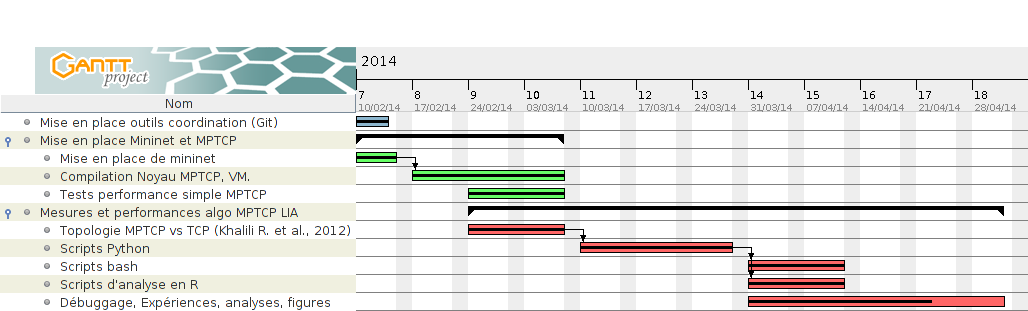
\includegraphics[width=1.2\textwidth]{../gantt/romain.png}
  \end{changemargin}
  \centering
  
  \caption{\textbf{Diagramme de Gantt de Romain Ly.}}
  \label{fig:gantt}
  
\end{figure}

\begin{itemize}
\item Mise en place du Git
\item Compilation noyau MPTCP dans la VM mininet et tests simples de routines
\item Topologie modifi�e de Khalili et al.
\item Scripts Python
  \begin{itemize}
  \item impl�mentation d'un parseur d'arguments
  \item int�gration de ping, iperf, iperf3, bwm-ng, sshd, tcpdump
    permettant le monitoring et l'�tude du r�seau
  \end{itemize}
\item Installation de TCP-reduce dans la VM pour v�rifier les options de la connexion TCP.
\item Scripts Bash pour g�n�rer de multiples simulations par l'interm�diaire de scripts Python
\item Scripts R pour analyse des r�sultats et figures
\item D�bogages des scripts
\item Exp�rimentations
  \begin{itemize}
  \item variation du nombre de sous flots, d�bits, latences, taille de
    fen�tre, etc.
  \end{itemize}
\end{itemize}


\subsection{Topologie \emph{fat-tree}}

\begin{figure}[!htb]
  \begin{changemargin}{-2.0cm}{0.5cm}
    \centering
    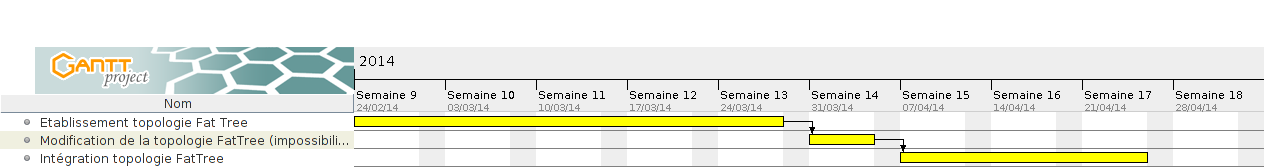
\includegraphics[width=1.2\textwidth]{../gantt/Simon.png}
  \end{changemargin}
  \centering
  
  \caption{\textbf{Diagramme de Gantt de Simon Ravier.}}
  \label{fig:gantt}
\end{figure}

\vspace{1cm}
\begin{tabular}{lp{12cm}}
  03/03 au 30/03 & �tablissement de la topologie FatTree\\
  31/03 au 06/04 & modification de la topologie FatTree (impossibilit� technique de r�aliser le premier mod�le)\\
  07/04 au 27/04 & Int�gration de la topologie FatTree dans
l'environnement de tests (configuration des h�tes, �tablissement des
tables de routage) et r�alisation des tests
\end{tabular}
\vspace{0.5cm}

\subsection{\'Ecriture d'un nouvel algorithme d'ordonnancement}
\begin{figure}[!htb]
  \begin{changemargin}{-2.0cm}{0.5cm}
    \centering
    \includegraphics[width=1.2\textwidth]{../gantt/KevinQuentin.png}
  \end{changemargin}
  \centering
  
  \caption{\textbf{Diagramme de Gantt Kevin Lam et Quentin Dubois}. }
  \label{fig:gantt}
\end{figure}

Analyse de la structure de l'impl�mentation :
	\begin{itemize}
		\item D�terminer globalement les fichiers � lire ;
		\item D�finir les headers et structures li�s � l'utilisation de mptcp.
	\end{itemize}\\

Lecture et Compr�hension du code :
	\begin{itemize}
   		\item Lecture de tous les fichiers contenus dans \$(SRC\_NOYAU)/net/mptcp ;
   		\item Lecture de certains fichiers contenus dans \$(SRC\_NOYAU)/net/sched ;
	   \item Lecture de tous les types/structures utilis�s ;
	   \item Relecture du code apr�s avoir compris tous le types/structures.
	\end{itemize}\\

D�finition des parties modifiables de l'ordonnanceur :
	\begin{itemize}
	   \item V�rifier les correspondances entre mptcp\_output.c et mptcp\_input.c ;
	   \item Voir si l'utilisation du contr�le de congestion (mptcp\_olia.c et mptcp\_coupled.c) a des effets de bord sur les sockets ;
	   \item Voir les diff�rences entre les diff�rents modes du path\_manager.
	\end{itemize}\\

Impl�mentation / Tests d'algorithmes pour l'ordonnanceur :
	\begin{itemize}
		\item Avec l'aide de Matthieu Coudron, modification dans
		\$(SRC\_NOYAU)/net/mptcp/mptcp\_output.c ;
	   \item Tests des impl�mentations avec le travail de Romain LY et comparer les r�sultats obtenus.
   	\end{itemize}\\


\clearpage
\section{Contexte technologique}
\label{sec:contexte-techno}
%// -*- coding: iso-8859-1 -*-

L'�laboration de MPTCP a �t� motiv�e par l'observation de l'existence
dans les r�seaux de plusieurs chemins entre deux machines A et
B. L'utilisation de ces diff�rents chemins entre les deux h�tes
pourrait �tre un atout non n�gligeable pour augmenter le d�bit de la
connexion et/ou la r�silience de la connexion si l'un des chemins
venaient � ne plus pouvoir acheminer les paquets (congestion, panne de
routeur, etc). De plus le multi-chemin permet d'�quilibrer la
r�partition des charges sur les sous-flots utilis�s. TCP n'a pas �t�
con�u pour exploiter plusieurs chemins d'o� la n�cessit� de concevoir
des protocoles multi-chemins comme MPTCP permettant d'utiliser les
chemins disponibles pour transmettre les paquets d'une connexion entre
A et B via les sous-flots connect�s.

Il existe d�j� plusieurs protocoles proposant d'utiliser plusieurs
chemins. Nous en citerons que deux: SCTP et ECMP. SCTP (\emph{Stream
  Control Transmission Protocol}) allie l'avantage de TCP et UDP
(utilisation de datagrammes) et permet de multiplexer les flux sur
plusieurs interfaces \cite{rfcsctp}. ECMP (\emph{Equal Cost
  MultiPath}) est un sous-protocole dans le cadre de divers protocoles
de routages (comme OSPF, TRILL, ...) et qui est utilis� dans les
\emph{data-centers}: lors d'une connexion entre deux h�tes, le routeur
peut transf�rer les paquets sur plusieurs meilleurs chemins � co�ts
\og �gaux \fg{} \cite{rfcecmp}. \\
Les inconv�nients de SCTP est la n�cessit� que tous les h�tes
terminaux puissent comprendre le protocole ; il est donc n�cessaire de
modifier la couche application pour pouvoir l'utiliser. De plus, les
\emph{middle boxes} (pare-feu, NAT, \ldots) ne reconnaissent pas le
protocole et rejettent donc tous les paquets SCTP. ECMP utilise les
routeurs pour conna�tre les chemins et l'augmentation de performance
li� � son utilisation n'est pas significative.

L'avantage principal de MPTCP est d'�tre r�trocompatible par rapport �
TCP.  Si un h�te n'est pas compatible avec MPTCP, la connexion
utilisera TCP r�solvant les probl�mes des \emph{middle boxes}. Le
scond avantage est qu'il est totalement transparent pour les routeurs,
c'est une connexion \emph{end to end}.


\subsection{Fonctionnement de MPTCP}
\label{subsec:fonctMPTC}

MPTCP utilise dans un premier temps une connexion TCP pour cr�er des
sous-flots similaires � TCP avec des chemins diff�rents. La couche TCP
est alors remplac�e par la couche MPTCP qui est divis�e en deux
parties (\fig{fig:mptcpstack}): la couche sup�rieure correspond aux
fonctions n�cessaires � MPTCP de fonctionner (d�couverte et gestion
des chemins, ordonnancement des paquets, contr�le de congestion) et la
couche inf�rieure correspond aux sous-flots �tablis.

\begin{figure}[!htb]
    \centering
    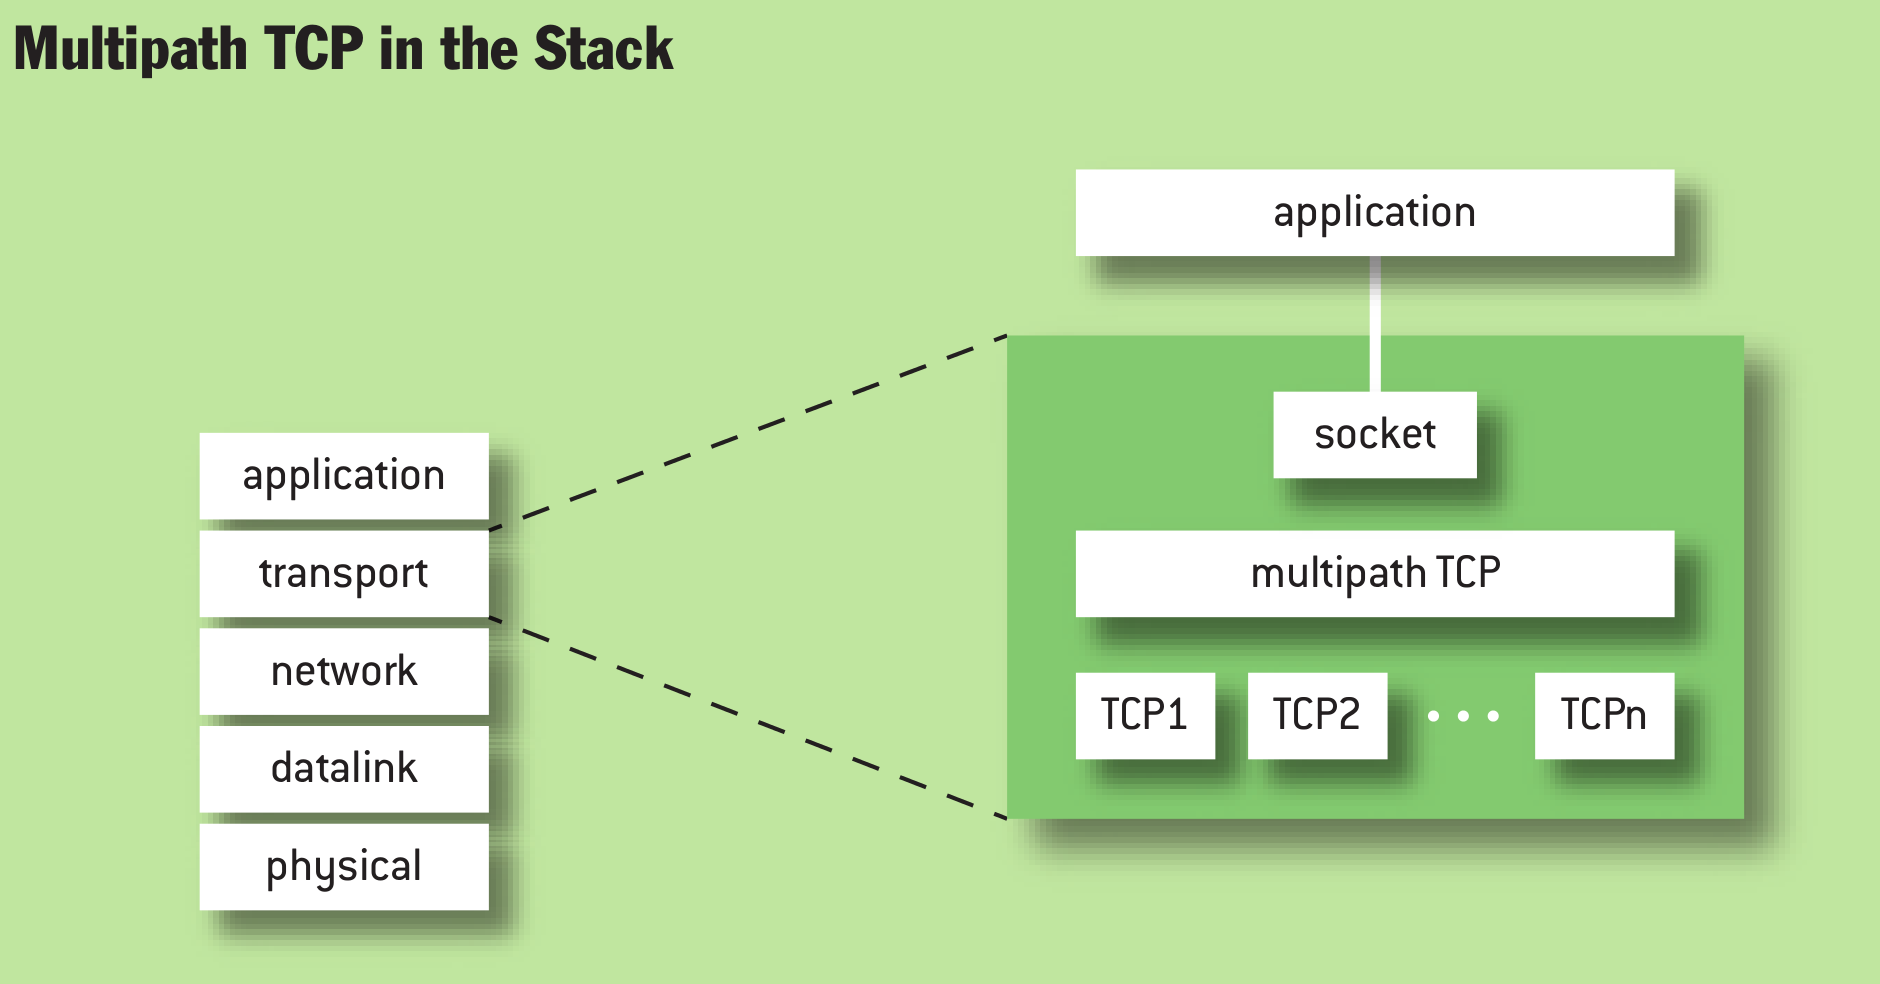
\includegraphics[width=0.8\textwidth]{../figures/mptcp_stack/mptcp_stack.png}
    \caption{\textbf{Sch�ma de la pile MPTCP} \cite{PB14}.}
  \label{fig:mptcpstack}
  
\end{figure}

MPTCP permet l'augmentation du d�bit de mani�re � ce qu'il soit
sup�rieur � une connexion TCP unique sur le meilleur des chemins
disponibles. Il permet aussi la r�silience de la connexion en cas de
panne ou de congestion, dans ce cas le trafic est alors r�parti et/ou
r�exp�di� sur les autres sous-flots sans la n�cessit� de r�tablir une
connexion TCP entre les deux terminaux. Cette approche permet de
r�partir les charges sur les ressources disponibles.

MPTCP impl�mente plusieurs fonctions pour contr�ler les sous-flots de
la connexion \cite{rfc6182}:
\begin{itemize}
\item le gestionnaire de chemin ou \emph{path manager} 
\item l'ordonnanceur de paquets ou \emph{packet scheduling} puis
\item le contr�leur de congestion  ou \emph{congestion controller}.
\end{itemize}

Le sous-flot prend en charge les segments de l'ordonnanceur pour
l'envoyer sur un chemin disponible. Le sous-flot agit comme une
connexion TCP classique et dispose de cette mani�re des fonctions de
ce protocole de transport assurant d'envoyer des paquets de mani�re
fiable et s�quenc�e. \`A la r�ception, le sous-flot envoie les
segments � la couche ordonnanceur de paquet pour le
r�assemblage. Mais, le r�assemblage est d'autant plus rapide si les
paquets re�us sont d�j� bien ordonn�s. Dans ce cas, avoir un
ordonnanceur, qui permet d'estimer le temps d'arriv�e des paquets
selon un sous-flot pour que le r�cepteur re�oive tous les paquets des
diff�rents sous-flots de fa�on ordonn�e permettrait d'augmenter les
performances de MPTCP. En effet, les donn�es dans le buffer seraient
trait�s plus efficacement. Cela affecte donc sur la quantit� de
donn�es pouvant \^etre envoy�es et/ou sur le nombre de sous-flots
exploitables.

Le gestionnaire des chemins est le m�canisme permettant de d�tecter et
d'utiliser les chemins disponibles par l'interm�diaire de multiples
adresses IPs dans les h�tes. Il signale l'existence d'adresses
alternatives et permet d'int�grer de nouveaux sous-flots � une
connexion MPTCP existante ou d'en enlever.

L'ordonnanceur des paquets d�coupe le flux de donn�es provenant de la
couche application en segments pr�ts � �tre envoy�s par l'un des
sous-flots. Il s�quence les segments et permet de r�associer les
segments pour r�ordonner les donn�es c�t� destinataire. L'ordonnanceur
d�pend des informations des chemins disponibles provenant du
gestionnaire de chemins \cite{rfc6356}.

Enfin, le contr�le de congestion est un outil essentiel qui permet
d'adapter le d�bit de chaque sous-flot et de d�finir si un chemin est
trop lent par rapport au meilleur sous-flot. Il permet aussi de
renvoyer l'information au gestionnaire s'il y a une panne.

\vspace{0,5cm}

Le contr�le de congestion n�cessite un algorithme performant pour que
l'utilisation de MPTCP � la place de TCP puisse effectivement
augmenter le d�bit de l'utilisateur sans influencer le d�bit des
autres utilisateurs sur les m�mes chemins, c'est � dire qu'il doit
garantir l'optimalit� de pareto (c'est � dire que l'allocation des
ressources est r�alis�e de mani�re ce qu'il soit impossible
d'augmenter le d�bit d'un utilisateur sans diminuer le d�bit d'un
tiers ou sans augmenter le co�t de la congestion. Il garantit aussi la
r�partition �quitable de la capacit� du lien entre les utilisateurs
\cite{pareto2013}).  L'algorithme de MPTCP est donc un point central
dans les performances de MPTCP sur le r�seau.

Lors des choix des sous-flots, l'algorithme doit effectuer un
compromis entre �quilibre des charges dans les diff�rents sous-flots
et r�activit� (\emph{responsiveness}) en cas de modification de la
latence des sous-flots ou de d�couverte de nouveaux chemins. Une
priorit� vers l'�quilibre des charges entra�ne l'envoi des donn�es sur
les meilleurs routes (selon la m�trique utilis�e, par d�faut la
latence du chemin) mais cela peut d�clencher un changement constant de
route produisant un effet de battement (\emph{flappiness}): si
plusieurs chemins poss�dent le m�me co�t, l'algorithme aura tendance �
changer plus souvent de chemins. Si la priorit� utilis�e est la
r�activit� (par augmentation de la taille de la fen�tre d'un des
sous-flot), l'utilisation de toutes les ressources disponibles peut ne
pas �tre optimale car on aura tendance � utiliser qu'un seul
sous-flot. Les param�tres de l'algorithme doivent �tre d�termin�s
efficacement pour r�partir les charges sur les sous-flots et ne pas
�tre agressif (augmentation trop rapide de la taille de la fen�tre sur
un des sous-flots) pour garantir l'optimalit� de Pareto
\cite{pareto2013}.

 Dans l'algorithme par d�faut, le crit�re privil�gi� par l'algorithme
est le RTT. Il serait int�ressant de modifier les caract�ristiques du
r�seau pour mesurer les performances de MPTCP sur le choix des chemins
utilis�s ou en cas de modification de chemins sur des crit�res de
latence, pertes, d�bit \ldots



\subsection{Utilisation r�elle de MPTCP}
\label{subsec:utilisation}

Dans la pratique, l'utilisation de MPTCP est difficile. L'utilisation
de plusieurs sous-flots ne garantie pas l'augmentation de d�bit. Pour
cel�, il est n�cessaire que les sous-flots empruntent des chemins
physiques diff�rents et aujourd'hui il n'est pas possible pour un
utilisateur de contr�ler le routage de ses paquets de bout en
bout. Une m�thode pour contourner le probl�me serait d'utiliser la
conjonction de MPTCP et de LISP (\emph{Locator/Identifier Separation
  Protocol}) qui permet de d�couvrir la diversit� de chemins existant
entre routeurs de bordures (A-MPTCP)
\cite{coudroncross2013}. 

Cependant il existe des cas o� MPTCP est utilisable � son plein
potentiel et suscite l'int�r�t : dans les datacenters et en
environnement mobile. Par l'interm�diaire d'une strat�gie de routage
par SDN (\emph{Software Defined Network}) par exemple OpenFlow, le
contr�leur peut �tablir des chemins diff�rents entre deux h�tes sur
tout son r�seau. Le transfert de donn�es au sein d'un datacenter
n�cessite des d�bits tr�s importants. L'utilisation de MPTCP pourrait
r�partir les charges entre les diff�rents noeuds. Des exp�riences sur
diff�rentes topologies de datacenter � haute densit� ont permis de
montrer que MPTCP �gale, voir surpasse m�me la performance d'un
ordonnanceur centralis� et est de surcroit plus robuste
\cite{raiciu2010}. En mobile, le terminal pourra utiliser le r�seau
3G/4G et le r�seau wi-fi environnant. MPTCP permettra de d�charger le
r�seau t�l�phonique de l'op�rateur tout en augmentant le d�bit et la
r�silience de la connexion.

\subsection{MPTCP et s�curit�}
\label{subsec:utilisation}

\`A l'heure d'Eric Snowden, l'utilisation de plusieurs sous-flots
pourrait �tre un avantage non n�gligeable en terme de s�curit�. Pour
pouvoir �pier une connexion entre A et B, il faudrait � l'attaquant de
pouvoir \emph{sniffer} les paquets qui sont �mis sur les sous-flots
utilis�s, c'est-�-dire sur autant de chemins physiques
diff�rents. L'int�r�t du multi-chemin prend alors tout son
sens. Cependant ce n'est pas le seul avantage, on peut r�fl�chir �
plusieurs moyens d'augmenter la s�curit� par l'utilisation du
multi-chemin conjoitement avec une modification des protocoles de
s�curit�. Voici quelques id�es personnelles d'une impl�mentation d'une
combinaison de MPTCP et de s�curit�.

\begin{itemize}
\item l'utilisation d'une m�thode de chiffrement par bloc de type CBC
  (\emph{Cipher Block Chaining}) compliquera la t�che de l'attaquant
  car il sera n�cessaire d'obtenir le bloc n-1 pour d�chiffrer le bloc
  n. Par exemple, AES-CBC est utilis� couramment dans des
  communications utilisant SSL/TLS. L'attaquant devra disposer de tous
  les paquets sans exception pour pouvoir d�chiffrer la totalit� du
  message en supposant qu'il poss�de la cl� secr�te.

\item De plus, si les protocoles de s�curit� sont conscients de
  l'utilisation de MPTCP, il pourrait y avoir une entente
  \emph{cross-layer}. Par exemple, en distribuant les informations des
  MAC (\emph{Message Authentication Code}) de chaque paquet entre les
  diff�rents sous-flots de mani�re � �viter les \emph{man in the
    middle}: sous flot 1 = message 1 + HMAC (message 2); sous flot 2 =
  message 2 + HMAC (message 1).  

\item Un autre exemple serait de n�gocier les cl�s pour le chiffrement
  de la communication d'un sous-flot (par exemple en utilisant IPSec)
  dans le sous-flot adjacent.
\end{itemize}


Dans tous les cas, il est donc n�cessaire que MPTCP dans une optique
s�curit� utilise au mininum deux sous-flots et donc de modifier
l'algorithme de congestion de MPTCP.  Dans une premi�re approche
simpliste, il serait int�ressant de forcer l'algorithme de MPTCP �
r�partir les paquets �quitablement sur plusieurs sous-flots, quitte �
diminuer les performances de MPTCP, c'est l'id�e que nous avons d�cid�
d'utiliser pour le nouvel algorithme d'ordonnancement.


\clearpage

\section{Analyse}
\label{sec:etat-avancement}
La partie Analyse sera �toff�e dans le rapport final par l'analyse des
r�sultats obtenus.

\section{Conception}
\label{sec:etat-avancement}


\subsection{Topologies virtualis�es}
\label{sec:conce:topologiesvirt}


Nous allons simuler des topologies openFlow en utilisant mininet. Les
switchs seront virtualis�s par openvSwitch (OVS) qui est install� par
d�faut dans l'image mininet. Pour utiliser le multi chemin, le noyau de 
MPTCP sera compil� dans la machine virtuelle et chaque h�te sera 
configur� de mani�re ad�quate pour pouvoir utiliser MPTCP.

Nous cr�erons et testerons les topologies virtuelles gr�ce � l'API
python.


\subsubsection{Multi-chemins simple}
\label{subsubsec:conception:multcihemin}
La topologie simple est compos�e de deux h�tes et de N switchs. Les N
switchs composeront les N chemins disponibles. Cette topologie simple
servira principalement au test de fonctionnement de MPTCP.

\subsubsection{FatTree}
\label{subsubsec:conception:fatTree}


Afin de tester MPTCP de mani�re r�aliste, nous avons simul� une
topologie FatTree, souvent utilis�e dans les datacenters qui sont les
premiers n�cessiteux des performances offertes par MPTCP. Cette
topologie repose sur le principe d'�tablir plusieurs liens physiques
entre deux �quipements r�seau, en l'occurrence des switchs. Tous les
switchs du r�seau ont le m�me nombre de ports; ils sont organis�s par
couches : une couche \og coeur\fg{}, une couche \og fronti�re \fg{} et
une couche \og h�tes\fg{}. Les couches h�tes et coeurs sont directement
connect�es � la couche fronti�re, mais pas entre elles. Chaque switch
de la couche coeur est connect� � chaque switch de la couche fronti�re
par de multiples liens. Le nombre de ports disponibles sur les
switchs coeurs est �quitablement r�parti entre chaque switch
fronti�re; ainsi, avec deux switchs coeurs et quatre switchs
fronti�res � 36 ports, on disposera de 9 liens entre chaque paire de
switchs de couches diff�rentes. Le reste des ports disponibles sur
les switchs fronti�res sont utilis�s pour y connecter les h�tes, �
raison d'un lien par h�te. Notons que deux �quipements d'une m�me
couche ne sont jamais interconnect�s.


\subsubsection{MPTCP vs TCP}
\label{subsubsec:conception:MPTCPvsTCP}

\begin{figure}[!htb]
  \centering
  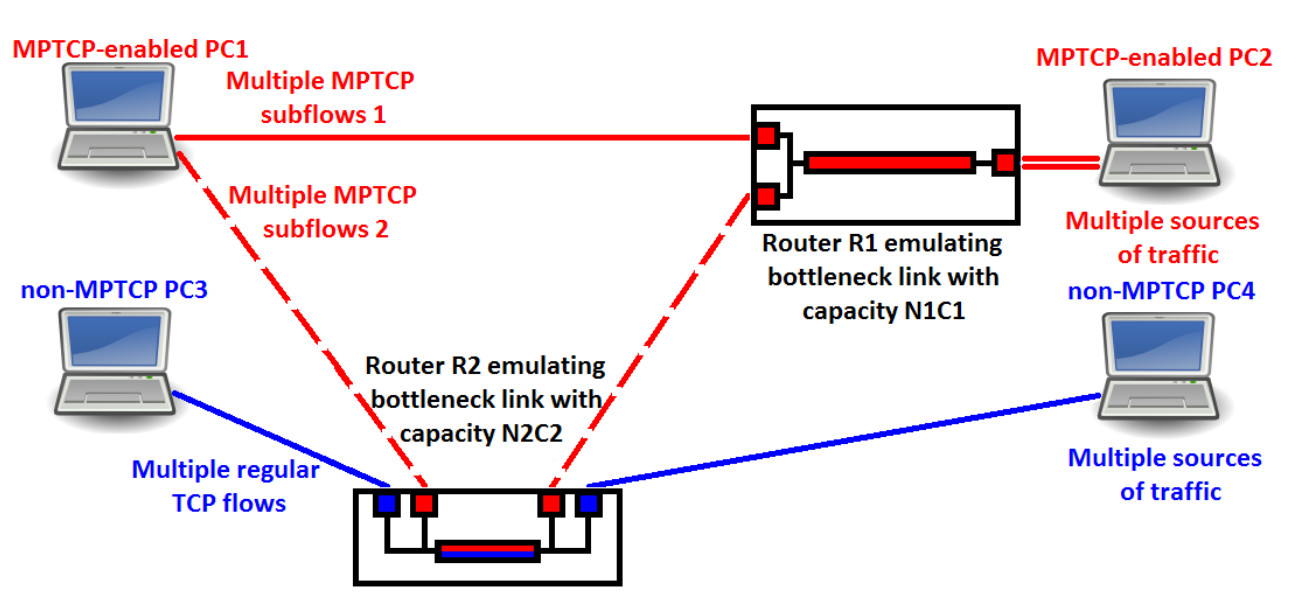
\includegraphics[width=0.6\textwidth]{../figures/khalili.jpg}
  \caption{\textbf{Testbed MPTCP vs TCP\cite{pareto2013}}.}
  \label{fig:khalili}
\end{figure}

Pour d�terminer les crit�res � respecter de l'ordonnanceur (celui par
d�faut, ou l'OLIA) et conserver les principes de MPTCP (�quitabilit�
avec les utilisateurs TCP et performances sup�rieures � TCP), nous
allons reproduire le \emph{testbed} utilis� dans l'article de Khalili
(\fig{fig:khalili}).


Si nous pouvons reproduire les r�sultats obtenus par Khalili avec
notre configuration, nous reproduirons le cas avec N1 utilisateurs
MPTCP et N2 utilisateurs TCP (voir \fig{fig:khalili2}).

\begin{figure}[!htb]
  \centering
  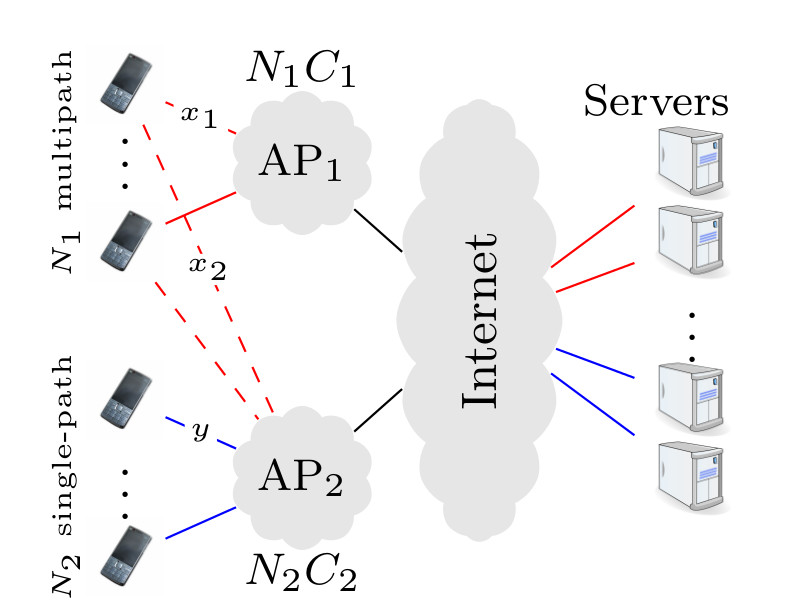
\includegraphics[width=0.4\textwidth]{../figures/khaliliB.jpg}
  \caption{\textbf{Testbed MPTCP vs TCP\cite{pareto2013}}. Les N1
    utilisateurs MPTCP (rouge) utilisent deux points d'acc�s pour se
    connecter � un serveur distant dont un qui est partag� avec les N2
    utilisateurs TCP (bleu).}
  \label{fig:khalili2}
\end{figure}

\subsection{Performances de MPTCP}
\label{sec:conce:perfMPTCP}

Pour mesurer les performances de MPTCP, nous allons faire varier les
propri�t�s de chaque sous-flot emprunt� en modifiant les chemins de
mani�re asym�trique. Le but est de cr�er des conditions de stress
qu'on pourra tester � la vol�e avec les diff�rents algorithmes g�rant
MPTCP (celui par d�faut, l'OLIA et le notre si celui-ci est
op�rationnel) et sur les diff�rentes topologies virtuelles construites.

Les contraintes appliqu�es auront comme crit�res la latence (crit�re
actuellement privil�gi� par l'ordonnanceur pour les choix de
sous-flots), la capacit�, le taux d'erreurs, la gigue, etc. Nous
testerons quelle est l'influence de ces param�tres sur le choix des
sous-flots par l'ordonnanceur.

\subsection{Conception algorithme s�curis�}
\label{sec:conc:algosec}

Le but est de rendre une connexion plus s�curis�e par la complexit� de
l'analyse des paquets de donn�es �chang�s entre deux
utilisateurs. Nous chercherons � faire une m�thode simple et non
performante pour effectuer des tests et savoir comment MPTCP r�agit au
nouvel algorithme de r�partition des paquets dans les sous-flots
TCP. Cette m�thode consiste � prendre le nombre de sous-flots total et
de r�partir les segments �quitablement entre les diff�rents
sous-flots. Le d�bit de chaque sous-flot correspondra au d�bit le plus
faible des sous-flots.  Cela reste une solution de l'objectif not�
dans le cahier des charges.

N�anmoins il sera n�cessaire d'avoir un algorithme plus
intelligent. En effet, il est n�cessaire d'avoir un meilleur
algorithme que celui expliqu� ci-dessus car la performance
pourrait �tre grandement affect�. Le d�bit pourrait �tre bien plus
faible qu'une connexion TCP classique sur le meilleur des chemins si
un des chemins a un d�bit beaucoup plus faible ou s'il est
congestionn�. Or m�me si nous voulons accro�tre la s�curit� il est
pr�f�rable d'avoir au moins le d�bit d'une connexion TCP simple. La
difficult� dans cette partie est de pouvoir adapter l'ordonnanceur
selon le nombre de sous-flots disponibles. Une id�e serait de r�partir
les charges de mani�re � que l'ordonnanceur de paquets n'envoie plus
de 50~+~$\varepsilon$~\% des segments � un unique sous-flot. Ce nombre
pourrait �tre variable selon d'autres param�tres comme le nombre de
sous-flots disponibles.


\subsection{Test de l'algorithme d'ordonnancement}
\label{sec:conc:ealgo}
L'�criture et le test de l'algorithme d'ordonnancement dans le noyau
linux peut s'av�rer une t�che difficile en si peu de temps. Pour
tester la validit� de notre algorithme d'ordonnancement, nous
r�fl�chissons � effectuer d'abord un \emph{proof of concept} en
utilisant directement python qui utilisera des fonctions de
\emph{callback} pour certaines fonctions du noyau n�cessaire �
MPTCP. On utilisera alors UDP pour la transmission des donn�es.

\clearpage

\section{\'Etat d'avancement}
\label{sec:etat-avancement}
\subsection[Outil de coordination: git]{Outil de coordination: git}
\label{subsec:etatavanc:git}
L'�tat des scripts utilis�es par l'�quipe est mise � jour par un
syst�me de version utilisant git
\url{https://github.com/Romain-Ly/PRES}.

\subsection[Compilation MPTC]{Compilation MPTCP\footnote{par M. Ly}}
\label{subsec:etatavanc:mininet-mptcp}

La mise en place du noyau linux MPTCP (v0.88) dans une VM de mininet
(v2.10) est � 100~\% termin�.

Les paquets debian pour l'installation du noyau MTPCP sur une VM de
mininet est disponible :
(\url{https://www.dropbox.com/sh/y4ykck8rg6908ps/7V3lsV6Ggg}).

Pour tester la r�ussite de l'installation, une topologie deux h�tes et
n switchs a �t� utilis�. L'utilisation de MPTCP montre un d�bit
sup�rieur lorsque l'on compare � la m�me exp�rience o� MPTCP a �t�
d�sactiv� dans le noyau.

\subsection[FatTree]{FatTree\footnote{par M. Ravier}}
\label{subsec:etatavanc:fattree}
Charg� de la conception du r�seau de test, ma premi�re pr�occupation a
�t� de ma�triser Mininet. Apr�s documentation, je me suis pench� sur
l'API Python offert par cet outil. Apr�s cette prise en main
concr�tis�e par quelques tests de connectivit� sur des topologies
simples, j'ai commenc� � coder ma propre topologie, un FatTree � 2
niveaux avec des switches � 36 ports. N'ayant pas trouv� de d�finition
formelle du FatTree, je me suis content� d'une instance particuli�re,
relativement simple mais permettant tout de m�me � MPTCP d'emprunter
plusieurs sous-flots diff�rents pour se rendre d'un h�te � l'autre.
Suite au travail de Romain, la prochaine t�che sera d'installer le
noyau MPTCP sur la machine virtuelle Mininet, de le configurer, puis
faire en sorte qu'il soit correctement utilis� dans notre r�seau
FatTree. J'effectuerai ensuite plusieurs tests de performance sur
cette topologie, probablement en collaboration avec Romain.

\subsection[Topologies virtualis�es]{Topologies
  virtualis�es\footnote{par M. Ly}}
\label{subsec:etatavanc:topologgie}

J'ai reproduit la topologie o� MPTCP est en concurrence avec un flux
TCP \cite{pareto2013}. Il reste � �tablir les tables de routage de
chaque h�te pour pouvoir tester les performances de MPTCP.


\subsection[Code MPTCP]{Code MPTCP\footnote{par M. Lam
    et M. Dubois}}
\label{subsec:etatavanc:mininet-mptcp}

Nous avons regard� les fichiers de MPTCP pour avoir une vision globale
de l'impl�mentation dans le noyau linux et essayer de d�terminer les
fichiers qui concernent l'ordonnancement des sous-flux.  Nous avons
ensuite essay� de d�terminer o� nous pouvions modifier le code afin
d'adapter l'ordonnanceur aux besoins du projet. Nous avons avanc� sur
cette phase de compr�hension du code mais il nous reste toujours �
savoir o� nous pouvons modifier le code sans rendre MPTCP non
fonctionnel ou non performant. Pour cela, il faudra tester sur des
topologies virtuelles simples et comparer les diff�rences de
performances. Bien s�r, dans les tests nous ne codons que des
ordonnanceurs idiots : ils effectueront uniquement une r�partition
�quitable des sous-flux sachant qu'ils ont tous le m�me d�bit.

\clearpage

\section{Compte rendu du projet}
\label{sec:compterendu}
\subsection[Outil de coordination: git]{Outil de coordination: git}
\label{subsec:etatavanc:git}
L'�tat des scripts utilis�es par l'�quipe est mise � jour par un
syst�me de version utilisant git
\url{https://github.com/Romain-Ly/PRES}.

\subsection[Compilation MPTC]{Compilation du noyau MPTCP (machine
  test)}
\label{subsec:etatavanc:mininet-mptcp}

Pour la r�alisation du projet, nous utilisons une machine virtuelle
ubuntu 13.04 (32 bits) o� mininet est install� et est pr�t pour
utilisation :
\url{https://bitbucket.org/mininet/mininet-vm-images/downloads}.

Nous avons compil� le noyau linux contenant MPTCP (v0.88) dans une VM
de mininet (v2.10). Les paquets debian pour l'installation du noyau
MTPCP sur une VM de mininet est disponible :
(\url{https://www.dropbox.com/sh/y4ykck8rg6908ps/7V3lsV6Ggg}).

Cepedant, l'architecture des machines pouvant �tre diff�rente, la VM
n'est pas fonctionnelle sur certaines des machines des membres du
projet. Par cons�quent, il est pr�f�rable de compiler soit m�me MPTCP
dans chaque machine. Le fichier ``.config'' est disponible sur le
git. La seconde option est d'utiliser ``apt-repository'' selon les
indications disponibles � cette adresse
\url{http://multipath-tcp.org/pmwiki.php/Users/AptRepository}.


\subsection{Topologie}
\label{subsec:CR:topologie}

Nous utilisons principalement deux topologies (A et B).

La topologie A est inspir� du \emph{testbed} de l'article de
R. Khalili \cite{pareto2013}, voir \fig{fig:topoMPTCP:A}. Nous avons
ajout�, � cette topologie, des routeurs priv�s entre le client et le
serveur \emph{MPTCP} pour disposer d'un nombre de sous-flots sup�rieur � deux.\\

\begin{figure}[!htb]
  \begin{changemargin}{-2.0cm}{0.5cm}
    \centering
    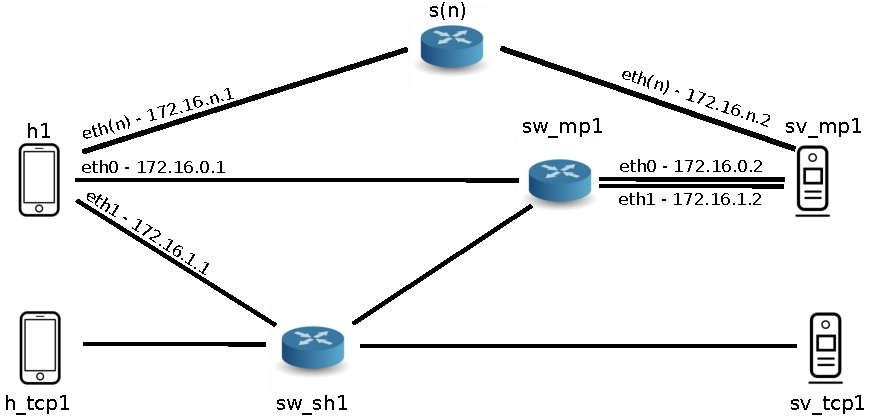
\includegraphics[width=0.7\textwidth]{../figures/mptcp_tcp/mptcp_tcp.pdf}
  \end{changemargin}
  \centering
  
  \caption{\textbf{Reproduction de la topologie de l'article de
      R. Khalili}. Le(s) \emph{switch(s)} ``S(n)'' ne sont pr�sent(s)
    que si le nombre de sous-flot est sup�rieure � deux. Pour n
    sous-flots, il y aura $n-2$ \emph{switchs} et $n-2$ liens
    suppl�mentaires. L'hyperviseur est connect� � tous les
    switchs. Pour se connecter via ssh aux h�tes, un \emph{switch} \og
    root \fg est cr�� et est connect� au \emph{switch} sw\_mp1 (non
    repr�sent� ici) voir utilisation CF linktobeadded.}
  \label{fig:topoMPTCP:A}
  
\end{figure}


La topologie B correspond au \emph{fat tree}.


\subsection{Performance de MPTCP sur mininet}
\label{sec:CR:perfMPTCP:base}

Apr�s la compilation du noyau, pour v�rifier le fonctionnement de
MPTCP nous avons mesurer le d�bit moyen en utilisant \emph{iperf} sur
la topologie A.

Les param�tres\footnote{param�tres par d�faut dans le noyau Linux}
utilis�s sont les suivants:


\vspace{1cm}
%\begin{tabular}{lp{\linewidth - 4cm}} 
\begin{tabular}{ll}
\textbf{Param�tre}& \textbf{Valeur}\\
\hline
MSS& 1460 octets\\
window size& 85,3 Koctets\\
d�lai par lien & 10 ms\\
Algorithme de congestion& LIA \cite{rfc6356}\\
\end{tabular}
\vspace{0.5cm}

Si nous fixons le MSS � 1460 octets, nous obtenons ce message
d'erreur:
\begin{verbatim}
  WARNING: attempt to set TCP maximum segment size to 1460, but got
  536
\end{verbatim}

Cependant, si nous analysons les paquets enregistr�s gr�ce � TCPdump,
nous observons que la taille maximal du MSS n�goci� pendant le
\emph{handshake} de la connexion MPTCP est de 1460 octets et que la
taille du MSS dans les paquets de donn�es est de 1428 octets.

\subsubsection{Un exemple de d�monstration}
\label{sec:CR:perfMPTCP:unique}

Ici nous allons prendre l'exemple d'une connexion avec deux sous-flots
� 100 Mbit/s. Voici la commande pour g�n�rer cet exemple:
\begin{verbatim}
sudo python ./pyMPTCP -O exp001_TC --bw 100 -t 30 -n 2 --mptcp --bwm_ng
\end{verbatim}

Pour les d�tails de l'activation de MPTCP dans le noyau et
l'utilisation des arguments des scripts python, une notice est donn�e
en Annexe 1: voir sections \ref{sec:annexe1:usepyth} page
\pageref{sec:annexe1:usepyth} et \ref{sec:annexe1:mininetParserargs}
page \pageref{sec:annexe1:mininetParserargs}.

\vspace{0.5cm}
Le d�lai (RTT) entre h1 et sv\_mp1 est de 44\,$\pm$\,11\,ms (mesur�
avec la commande ping), ce qui correspond bien au d�lai n�cessaire
pour traverser deux liens. La moyenne ici tient compte du d�lai du
premier paquet qui est envoy� vers le contr�leur qui va �tablir le
chemin vers le serveur\footnote{Il pourrait �tre n�cessaire d'enlever
  le d�lai de ce premier paquet dans une version future.}.

L'argument ``-\,-bwm-ng'' permet de lancer Bandwidth Monitor
NG\footnote{\url{http://www.gropp.org/?id=projects&sub=bwm-ng} }
(bwm-ng) et de mesurer plusieurs param�tres comme le nombre d'octets,
de paquets, le d�bit entrant ou sortant passant par chacune des
interfaces sond�es. La Figure \ref{fig:MPTCP-perfbwm-ng} montre le
d�bit entrant c�t� serveur pour ses deux interfaces, nous observons
que pour deux sous-flots aux capacit�s identiques, le d�bit mesur� est
quasi identique (une diff�rence de quelques paquets est observ�e).

\begin{figure}[htb]
    \centering
    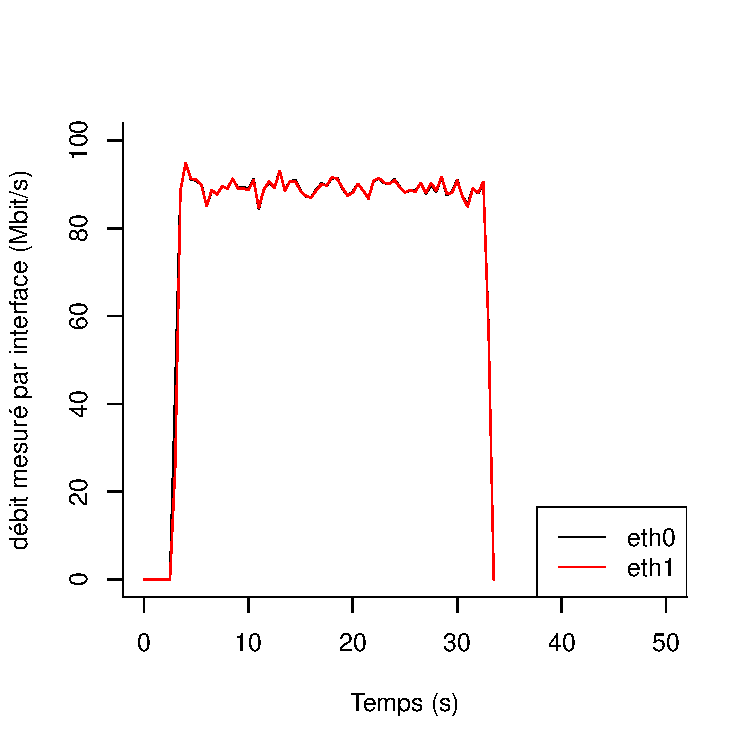
\includegraphics[width=0.7\textwidth]{../figures/bw-single.pdf}
    \caption{\textbf{D�bit entrant c�t� serveur.} �chantillonage : 2\,Hz.}
  \label{fig:MPTCP-perfbwm-ng}
\end{figure}

Pour mesurer le d�bit total g�n�r�, nous moyennons les d�bits totaux
mesur�s toutes les secondes par \emph{iperf} entre 5 secondes apr�s le
d�but de la connexion et 1 seconde avant la fin de la connexion. Nous
obtenons, c�t� serveur et pour cet exemple, un d�bit maximal de
168\,Mbit/s ce qui est attendu par les mesures de d�bit \emph{via}
bwm\_ng.


\subsubsection{Variation du d�bit maximal par lien}
\label{sec:CR:perfMPTCP:nsousflots}

Pour conna�tre les limites de la capacit� de notre simulation, nous
faisons varier le d�bit maximal par sous-flot, ainsi que le nombre de
sous-flots dans la topologie A.

\begin{figure}[htb]
    \centering
    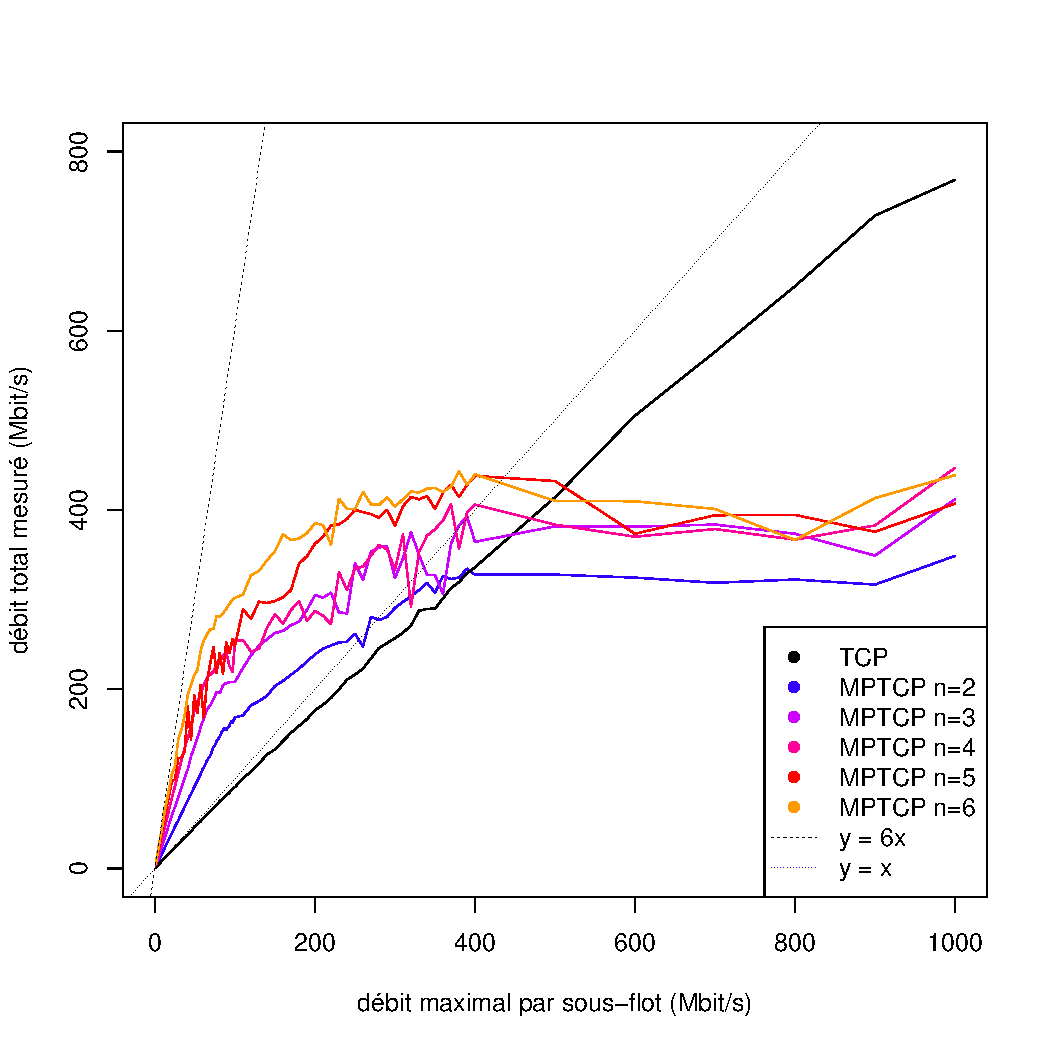
\includegraphics[width=0.7\textwidth]{../figures/bw-coupled.pdf}
    \caption{\textbf{D�bit total mesur� en fonction du d�bit maximal
        par sous-flot.} Les d�bits sont mesur�s avec \emph{iperf} pour
      une connexion TCP classique et une connexion MPTCP contenant de
      2 � 6 sous-flots.}
  \label{fig:MPTCP-perf-subflow-bw}
\end{figure}

Nous observons une phase lin�aire o� l'augmentation du d�bit par lien
ou l'augmentation du nombre de sous-flots augmente lin�airement le
d�bit total obtenu c�t� serveur. Cette phase situ�e en dessous des
100\,Mbit/s par lien correspond au but de MPTCP : augmentation du
d�bit. Cependant, les performances d�croissent rapidement et tombent
sous les performances d'une simple connexion TCP ce qui est contraire
� la nature m�me de MPTCP \cite{rfc6182}.

Ce probl�me pourrait �tre expliquer par l'utilisation non optimale de
la capacit� des sous-flots. Le \emph{bandwidth delay product} (BDP)
implique une taille minimale du tampon de r�ception. Pour un d�bit de
1000\,Mo et un RTT de 44\,ms, on obtient une taille minimale de tampon
de 5,5\,Mo. Sachant que le tampon de r�ception est partag� pour tous
les sous-flots d'une connexion MPTCP \cite{rfc6824}, la taille
minimale du tampon de r�ception doit suivre cette formule :

\begin{equation}
  \label{eq:MPTCP:buffer}
  buffer\_size \geqslant max(\{RTT_i\}_{i \in [1,n]})*\sum_{i \in [1,n]} Bandwidth_{\{i\}}
\end{equation}

C'est � dire que la taille du tampon de r�ception doit �tre le produit
du RTT maximal parmi tous les sous-flots et le d�bit total de tous les
sous-flots r�unis. Cette taille de tampon garantit l'utilisation
optimale du lien lorsque des paquets n�cessitent d'�tre retransmisent
sur des sous-flots aux d�lais lents. Dans notre simulation, il n'y a
pas de perte de paquet, la valeur minimale correspond au BDP le plus
�lev�.

Pour les m�mes propri�t�s de liens, avec deux sous-flots, nous
obtenons une taille minimale de 11\,Mo. Mininet modife automatiquement
les tampons au lancement de la topologie et les valeurs utilis�es sont
les suivantes:

\begin{verbatim}
net.core.wmem_max = 16777216
net.core.wmem_default = 163840
net.core.rmem_max = 16777216
net.core.rmem_default = 163840
net.ipv4.tcp_wmem = 10240	87380	16777216
net.ipv4.tcp_rmem = 10240	87380	16777216
net.ipv4.tcp_mem = 19326	25768	38652
\end{verbatim}

Nous observons que le tampon maximal pouvant �tre allou� par socket
est de 16\,Mo environ ce qui est largement sup�rieur � la taille
requise. De plus en augmentant la taille du tampon, nous n'observons
pas d'augmentation de performances alors qu'en le diminuant, nous
observons une diminution du d�bit mesur�
Fig. \ref{fig:mptcp:windowscale}.

\begin{figure}[!htb]
  \begin{changemargin}{-2.0cm}{0.5cm}
    \centering
    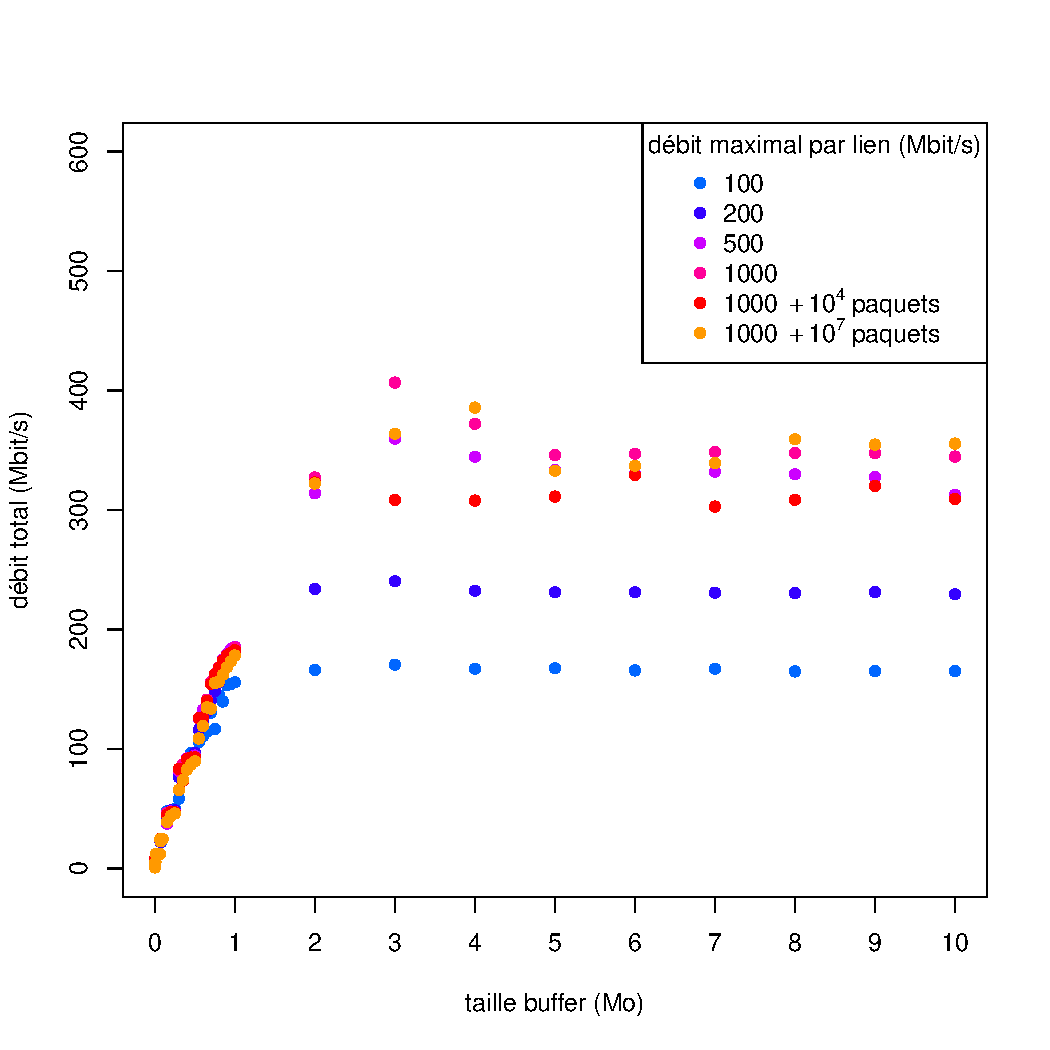
\includegraphics[width=0.7\textwidth]{../figures/ws.pdf}
  \end{changemargin}
  \centering
  
  \caption{\textbf{D�bit mesur� en fonction de la taille de la
      fen�tre}. La taille maximmale de la fen�tre TCP est modifi�e
    avec l'argument '-w' avec \emph{iperf}. La taille obtenue est
    �trangement de deux fois sup�rieure � la taille demand�. Le nombre
    de paquets correspond � la taille maximale de la queue des
    routeurs.}
  \label{fig:mptcp:windowscale}
  
\end{figure}

Nous obtenons les m�mes r�sultats en modifiant la taille maximale de
la queue des routeurs ou en modifiant les valeurs dans le noyau (voir
\ref{sec:annexe1:windowsize} page \pageref{sec:annexe1:windowsize})
que ce soit les param�tres minimum, par d�faut et maxium
d'\emph{auto-tuning} de TCP (\emph{net.ipv4}) ou les valeurs maximales
ou par d�faut pour tous les type de connexions (\emph{net.core}). Une
v�rification de la charge CPU global avec \emph{htop} ne montre pas
une saturation des processeurs (environ 15\,\% d'utilisation)
cependant, il reste � impl�menter \emph{cpuacct} pour v�rifier la
charge CPU par conteneur.


En effectuant des
recherches\footnote{\url{https://github.com/mininet/mininet/wiki/Introduction-to-Mininet\#what-are-mininets-limitations}}\footnote{\url{https://mailman.stanford.edu/pipermail/mininet-discuss/2014-January/003901.html}},
il semblerait que la limite du d�bit est li� aux n\oe uds Open vSwitch
sur Ubuntu 13.04, ce qui pour une dizaine de liens limite la capacit�
� 100 Mbit/s. C'est pourquoi, nous utiliserons des d�bits de 10 Mbit/s
environ pour les prochaines exp�riences.

\clearpage

Une partie de ce projet consiste dans un premier temps en l'�tude du
code de MPTCP et de la compr�hension de son fonctionnement, puis de
l'impl�mentation d'un nouvel ordonnanceur de notre choix. Apr�s
discussions, nous avons d�cid� de placer deux personnes sur l'�tude du
code de MPTCP car il nous semblait important d'avoir une bonne
connaissance du fonctionnement du code et des principales structures
pour pouvoir impl�menter un nouvel algorithme d'ordonnancement.

\subsection{Etude de  l'algorithme de MPTCP}
 	\subsubsection{Explication de l'ordonnanceur}
 	Lors de l'�tude du code de MPTCP, nous avons �tudi�
        l'ordonnanceur d�j� impl�ment�. L'ordonnanceur de MPTCP tient
        dans la fonction get\_available\_subflow(), qui se trouve dans
        (\$SRC NOYAU)/net/mptcp/mptcp.output.c. Cela nous a �t�
        confirm� par Matthieu Coudron lorsqu'il a choisi
        l'ordonnanceur � impl�menter. Cette fonction retourne la
        socket sur laquelle sera envoy�e le prochain segment de
        donn�es et d�finit la taille du Maximum Segment Size
        (MSS). Nous allons vous expliquer comment marche cet
        algorithme. Mais pour cela il faut connaitre d'avance les
        structures principales que nous allons vous expliquer avant de
        commenter l'ordonnanceur.
        \\
 	Tout d'abord la structure mptcp\_cb signifie \emph{MPTCP
          control block} c'est la pierre angulaire de MPTCP. Elle est
        utilis�e dans pratiquement toutes les fonctions de
        MPTCP. Cette structure permet de superviser les diff�rents
        sous-flots utilis�s pour une connexion MPTCP. Elle permet
        aussi de d�cider s'il faut ouvrir ou fermer un sous-flot, elle
        r�ordonne les donn�es re�ues afin que l'application qui a
        besoin de ces donn�es les obtienne dans le bon ordre.
        \\
 	La structure sock (socket) et la structure sk\_buff (socket
        buffer) sont les m�mes que dans TCP. La socket permet de cr�er
        une liaison entre les machines : elle d�tient les informations
        n�cessaires � la transmission des donn�es; quant au socket
        buffer, elle permet de d�finir ce que doit envoyer une socket
        et permet de faire un tri sur les donn�es re�ues gr�ce aux
        timestamps.  L'ordonnanceur impl�ment� dans MPTCP utilise,
        comme dans notre impl�mentation, le Smoothed Round Trip Time
        (SRTT) pour d�terminer quelle socket enverra les donn�es. De
        ce fait, si le SRTT est petit, l'ordonnanceur utilisera plus
        souvent cette socket. C'est ce qui cr�e une faiblesse dans la
        s�curit� de la transmission alors qu'avec MPTCP, comme il y a
        plusieurs chemins, la complexit� peut �tre accrue s'il y a un
        �quilibrage dans l'envoie des donn�es entre les sous-flots.
        \bigbreak
        Nous allons maintenant nous int�resser � la fonction get\_available\_subflow() qui est l'ordonnanceur.\\
        L'algorithme se d�roule de la fonction suivante:
 	 \begin{itemize}
         \item Tout d'abord, il y a une v�rification sur le nombre de
           sous-flots ouverts dans la connexion MPTCP. Il est possible
           de r�cup�rer cette valeur gr�ce � la structure mptcp\_cb(
           $mpcb->cnt\_subflows$ ). On effectue ce test au pr�alable
           dans le cas o� il n'y aurait qu'un seul sous-flot, au quel
           cas, il suffit de renvoyer l'unique socket s'il est
           disponible. Pour tester la disponibilit� d'une socket, la
           fonction \emph{mptcp\_is\_available()} existe d�j�. Elle
           v�rifie qu'elle peut envoyer (v�rification des champs de la
           socket), que la connexion est totalement �tablie, que la
           socket soit �ligible et, que sa fen�tre d'envoi est
           suffisante. Si la fonction renvoie \emph{true} alors le
           sous-flot peut �tre �ligible pour envoyer des donn�es. On
           peut r�cup�rer les sockets via la structure
           $mpcb->connection\_list$ qui liste les sockets associ�es
           aux sous-flots.
         \item Sinon on regarde toutes les sockets associ�es � la connexion MPTCP et on distingue trois types de sockets: les backup sockets, lowpriority sockets et la meilleure socket.\\
           Dans cet algorithme, il y a des sockets qui ont une
           priorit� basse et qui ne serviront que s'il n'existe pas de
           sockets avec une priorit� plus grande que cette
           priorit�. C'est ce qu'on appelle les lowpriority
           sockets. Parmi toutes les sockets, on choisit celle qui a
           le plus petit SRTT. Et on la stocke dans la variable
           \emph{lowpriosk}. Bien qu'elle soit nomm�e lowpriority,
           elle a une fonction de backup mais c'est une socket
           �ligible contrairement � la backup socket.
         \item Si il y a d'autres sockets qui n'ont pas une faible priorit�, on compare le SRTT de ces sockets et on garde la socket avec le RTT le plus faible. Elle est stock�e dans la variable \emph{bestsk}.\\
           Il y a aussi une backup socket qui sert au cas o� aucune
           des sockets d�crites ci-dessus ne peuvent envoyer un
           segment de donn�es : c'est le dernier recours car celle-ci
           est d�sign�e alors qu'elle ne permet pas la r�injection de
           donn�es. Elle sera stock�e dans la variable
           \emph{backupsk}.
\item Maintenant que nous avons d�fini les diff�rents types de
  sockets, il faut savoir sur laquelle des trois sockets on va envoyer
  les donn�es; Si il n'y a que des sockets de backup, on envoie les
  donn�es sur la \emph{lowpriosk}. Sinon on envoie les donn�es sur
  la \emph{bestsk} si elle existe. Et s'il n'y a pas de
  \emph{bestsk}, on utilise \emph{backupsk}.
\end{itemize} 

 	\subsection{Choix de l'ordonnanceur}
        Pour le projet, il fallait choisir et impl�menter un nouvel
        ordonnanceur. Nous avions �mis plusieurs hypoth�ses pour ce
        nouvel algorithme. En accord avec les encadrants, il a �t�
        d�cid� de juste utiliser le SRTT des sockets pour faire notre
        impl�mentation.  \bigbreak Dans un premier temps, nous avons
        pens� impl�menter un algorithme assez simpliste mais qui
        permettait d'augmenter la s�curit� contre les attaques de type
        \emph{Man In The Middle}. C'est � dire que notre algorithme
        allait envoyer les segments de mani�re �quitable sur chaque
        sous-flot permettant l'envoi de donn�es. Cet algorithme avait
        pour vocation de rendre plus difficile la r�cup�ration
        d'informations en �coutant un sous-flot car avec l'algorithme
        actuel, si un attaquant voulait r�cup�rer un maximum
        d'informations, il lui suffisait d'�couter le sous-flot qui a
        le SRTT le plus faible. C'est ce que nous voulions �viter avec
        notre algorithme. Cependant apr�s de plus amples r�flexions,
        nous avons remarqu� que notre algorithme avait un grand nombre
        de d�fauts.
        \\
        En effet, MPTCP a �t� d�velopp� afin d'am�liorer les
        d�bits. Cet algorithme n'aurai pas eu l'effet escompt� si le
        d�bit d'un sous-flot �tait vraiment faible compar� aux autres
        sous-flots alors, ce qui influencerait sur les performances de
        MPTCP. C'est pourquoi cet algorithme n'a pas �t� choisi.
        \bigbreak Un compromis entre s�curit� et performance est
        n�cessaire pour que l'utilit� de MPTCP soit avantageuse par
        rapport � TCP. Il nous a �t� propos� de s�lectionner les
        \emph{k} meilleurs sous-flots d'un point de vue du SRTT et de
        faire un Round-Robin sur ces k sous-flots. \emph{k} �tant
        laiss� � notre appr�ciation. Cet algorithme est le meilleur
        compromis trouv� car il permet de ne pas envoyer de donn�es
        sur un sous-flot si son SRTT est trop grand, ce qui permet de
        garder une certaine rapidit� dans la transmission de donn�es
        et de garder une certaine s�curit� car le trafic passe de
        mani�re �quitable sur les \emph{k} meilleurs sous-flots.

        \subsection{Impl�mentation de l'ordonnanceur}
        Afin de pouvoir stocker les \emph{k} meilleurs sous-flots, on
        avait 2 choix.
\begin{itemize}
\item Soit un tableau.
\item Soit une liste chain�e.
\end{itemize}
Apr�s en avoir discut� entre nous, nous avons d�cid� d'utiliser une
liste chain�e car les listes chain�es permettent une plus grande
flexibilit� de manipulation. Nous avons donc d�clar� dans
\emph{mptcp.h}, une structure:
\begin{verbatim}
struct selected_sk{
  struct sock *sk;
  struct selected_sk *next;
};
\end{verbatim}
Cette structure permet de pointer sur une socket et de d'avoir un lien
vers la socket suivante ce qui permet de naviguer tr�s facilement
entre les diff�rentes sockets s�lectionn�es. Ce qui est tr�s utile
pour le Round-Robin.  \bigbreak
Une fois que l'on avait d�clar� cette structure, il fallait aussi impl�menter des fonctions afin de pouvoir faire une liste chain�e en fonction des RTT. Notre liste chain�e sera organis�e de telle sorte:\\
On aura une \emph{selected\_sk} qui sera appel�e \emph{bssk}. C'est la
"best selected socket". Ce sera la socket s�lectionn�e qui aura le
meilleur RTT, puis son attribut next pointera sur la deuxi�me socket
avec le meilleur RTT. Et la $k^{eme}$ socket aura pour \emph{next} la
\emph{bssk}. Cela formera une boucle.
Les fonctions cr��es sont:\\
\begin{itemize}
\item \emph{static void ssk\_insertion\_sort(struct selected\_sk *bssk, int ssk\_size);} : qui permet de faire en sorte que la liste chain�e soit tri�e en fonction du Smoothed RTT (SRTT) des sockets.
\item \emph{static u32 ssk\_max\_srtt(struct selected\_sk *bssk);} : permet de retourner la valeur maximale du SRTT de la liste chain�e, c'est � dire le RTT de la socket qui a pour\emph{next} la bssk pass�e en argument.
\item \emph{static int belongto\_ssk(struct sock *sk, struct
    selected\_sk *bssk, int ssk\_size);} : permet de savoir si la
  socket sk pass�e en argument appartient � la liste chain�e.
\item \emph{static struct selected\_sk *bssk\_prev(struct
    selected\_sk *bssk);} : permet d'obtenir la socket ayant le plus
  grand SRTT de la liste chain�e. C'est la socket pr�c�dent la
  \emph{bssk}.
\item \emph{static void ssk\_checkup(struct sk\_buff *skb, struct
    selected\_sk *bssk, int ssk\_size);} : permet de retirer les
  sockets de la liste chain�e si elles ne sont pas capable d'envoyer
  des donn�es ($!mptcp\_is\_available(it->sk, skb, \&this\_mss)$) et
  si on a d�j� mis dans la queue de la socket le buffer \emph{skb}
  ($mptcp\_dont\_reinject\_skb(tp, skb)$).
\end{itemize}
O� $ssk\_size$ est le nombre de socket qui forme la liste chain�e.
\bigbreak
Avec ces fonctions nous pouvons cr�er la fonction principal que l'on placera dans \\
\emph{static struct sock *get\_available\_subflow(struct sock
  *meta\_sk, struct sk\_buff *skb,
  unsigned int *mss\_now); }\\
Nous allons maintenant expliquer comment fonctionne la fonction
principale: On v�rifie tout d'abord si tous les sockets de la liste
chain�e ont envoy� une fois (si elles existent toujours) et si oui, on
recalcule la liste chain�e.  Dans cette boucle qui permet d'�tablir
cette liste chain�e, on teste chaque socket si elle est disponible. Si
la socket a un meilleur SRTT ou qu'il reste de la place dans les k
meilleures sockets, on rajoute cette socket dans la liste. Pour cela,
une insertion est effectu�e en gardant la liste tri�e. Par contre, si
le SRTT est plus grand que ceux de la liste chain�e et qu'il y a d�j�
k sockets, on passe � la socket suivante.
\subsection{Debug de l'ordonnanceur impl�ment�}
On a impl�ment� un ordonnanceur mais il faut le tester dans les
topologies virtualis�es. Divers probl�mes ont �t� rencontr�s avec la
machine virtuelle mininet lorsque l'on a voulu utiliser MPTCP. En
effet, � cause de l'h�t�rog�n�it� de nos machines physiques, nous
devions chacun faire nos propres corrections pour compiler le noyau
(probl�mes de drivers � la compilation, de machine virtuelle, de
package openvswitch). Mais apr�s les avoir corrig�s, nous avons une
impl�mentation pas encore fonctionnelle. En effet, lors de l'ex�cution
du script python de test de MPTCP, on obtient un "kernel panic" sur la
fonction d'ordonnancement. Cette fonction est toujours en correction,
� l'aide de User Mode Linux (UML). Nous esp�rons qu'elle sera
op�rationnelle d'ici la soutenance et que l'on pourra mener quelques
tests de performances sur notre impl�mentation.

\clearpage

\clearpage

\section{Conclusions}
\label{sec:conclusions}

Au cours de ce projet, nous avons :

\begin{itemize}
\item compil� le noyau MPTCP dans une machine virtuelle contenant
  mininet;
\item cr�� une plateforme de tests par des scripts python et bash;
\item test� le fonctionnement de MPTCP sur une topologie simple et sur
  la topologie \emph{fat-tree};
\item test� les capacit�s et les limites de la virtualisation de
  r�seaux;
\item puis mesur� les performances de MPTCP sur des liens � d�lai
  variables;
\item enfin, nous avons �crit un nouvel algorithme d'ordonnancement;
\item et nous avons compil� le noyau avec ce nouvel algorithme
\end{itemize} (bien qu'il ne soit pas encore op�rationnel).

\section{Perspectives}
\label{sec:perspectives}
Le sujet est tr�s int�ressant et les pistes pour continuer le projet
sont nombreuses.

Dans un premier temps, il serait profitable de terminer les scripts de
base en int�grant des moyens pour mesurer la charge CPU par conteneur
(\emph{cpuacct}) ou de mesurer le RTT par la connexion TCP. Ensuite,
il serait utile de faire varier d'autres param�tres comme la
probabilit� d'erreur, la gigue sur chacun des liens pour ensuite,
effectuer des exp�riences sur des liens congestionn�s o� plusieurs
utilisateurs sont en concurrence pour la ressource. Ces tests
stringents seront utiles pour mesurer la performance des algorithmes
contenus dans le noyau et pour les comparer avec le nouvel algorithme.

Concernant l'impl�mentation de l'ordonnanceur qui est toujours en
cours de correction, terminer cet algorithme et comparer les r�sultats
des deux algorithmes serait b�n�fique : modifier, par la suite, les
crit�res d'ordonnancement selon les r�sultats obtenus avec mininet
pour l'optimiser.





\section{Remerciements}
\label{sec:remerciements}

Ce projet a �t� r�alis� dans le cadre du Master I R�seau, �
l'Universit� Pierre et Marie Curie.

Nous tenons � remercier Stefano Secci pour nous avoir permis de
r�aliser ce projet.  

Et nous remercions Yacine Bencha�b et Matthieu Coudron pour les
discussions autour du projet.

%// -*- coding: iso-8859-1 -*-

\section{Annexe1}
\label{sec:annexe1:annexe1}


\subsection{Utilisation des scripts pythons}
\label{sec:annexe1:usepyth}

\subsubsection{Activation MPTCP}
\label{sec:annexe1:MPTCP}


Il y a deux fichiers qui nous int�ressent:
\begin{verbatim}
/proc/sys/net/mptcp_path_manager
/proc/sys/net/mptcp_enabled
\end{verbatim}

Le fichier enabled permet d'activer (\emph{1}) ou de d�sactiver
(\emph{0}) MPTCP sur la machine.

Le fichier path\_manager influence sur la m�thode d'annonce des
sous-flots. Deux valeurs nous int�ressent: \emph{fullmesh}, et
\emph{default}. La valeur \emph{default}, il n'y a pas d'annonces des
sous-flots disponibles tandis que \emph{fullmesh} permet la cr�ation
d'un \emph{mesh} de sous-flots parmi tous ceux disponibles.

Pour modifier la valeur du fichier, il suffit d'utiliser sysctl en utilisant la forme ``nom=valeur''

\begin{verbatim}
sudo sysctl -w net.mptcp.mptcp_path_manager=fullmesh
sudo sysctl -w net.mptcp.mptcp_enabled=1
\end{verbatim}

Attention, selon les choix lors de la compilation du noyau, la valeur
par d�faut du path\_manager peut �tre mise sur ``default''.

\subsubsection{Choix de l'algorithme congestion}
\label{sec:annexe1:MPTCPcongestion}
Pour choisir l'algorithme de congestion, il est n�cessaire de modifier
le fichier suivant :

\begin{verbatim}
/proc/sys/net/ipv4/tcp_congestion_control
\end{verbatim}

Pour l'algorithme LIA:
\begin{verbatim}
sudo sysctl -w net.ipv4.tcp_congestion_control=coupled
\end{verbatim}

Pour l'algorithme OLIA:
\begin{verbatim}
sudo sysctl -w net.ipv4.tcp_congestion_control=olia
\end{verbatim}

Pour l'algorithme par d�faut:
\begin{verbatim}
sudo sysctl -w net.ipv4.tcp_congestion_control=cubic
\end{verbatim}

Pour afficher les algorithmes disponibles:
\begin{verbatim}
sudo sysctl net.ipv4.tcp_available_congestion_control
\end{verbatim}

L'ordonnanceur par d�faut est choisi � la compilation du noyau.

\subsubsection{Taille de la fen�tre}
\label{sec:annexe1:windowsize}

Pour modifier la taille maximale de la fen�tre de r�ception
(\emph{rmem}) et d'envoi \emph{wmem}, il faut modifier les fichiers
suivants:

\begin{verbatim}
/proc/sys/net/core/wmem_max
/proc/sys/net/core/rmem_max
/proc/sys/net/core/rmem_default
/proc/sys/net/core/rmem_default
\end{verbatim}

Pour une taille \emph{buffer} maximale de $\sim$16\,Mo:
\begin{verbatim}
sysctl -w net.core.wmem_max=16777216
sysctl -w net.core.rmem_max=16777216
\end{verbatim}

Pour modifier les valeurs par d�fauts :
\begin{verbatim}
sysctl -w net.core.rmem_default=163840
sysctl -w net.core.wmem_default=163840
\end{verbatim}

Pour modifier les valeurs d'\emph{auto-tuning}:
\begin{verbatim}
sysctl -w net.ipv4.tcp_wmem='4096 16384 4194304'
sysctl -w net.ipv4.tcp_rmem='4096 87380 6291456'
\end{verbatim}
Les valeurs correspondent respectivement � la taille minimale, par
d�faut et maximale du buffer allou� (en octets) par socket TCP. La
taille maximale ne peut d�passer celle indiqu�e dans \emph{net.core.}


\subsection{Lancement scripts python}
\label{sec:annexe1:python}

Les fichiers permettant de lancer la topologie et d'ex�cuter les tests
se nomment en commen�ant par ``pyMPTCP'' et se situent sur le git pour
l'instant dans ``./mininet/python/TCPvsMPTCP''

\begin{verbatim}
pyMPTCP.py
pyMPTCP_parser.py
pyMPTCP_topo.py
pyMPTCP_options.py
\end{verbatim}

pyMPTCP.py contient le \emph{main} et doit �tre modifi� pour choisir
la topologie (objet \emph{topo} dans la fonction \emph{main} et objet
\emph{net} dans la fonction \emph{runMPTCP}).

pyMPTCP\_topo.py contient les d�finitions des topologies utilis�es. La
classe \emph{Topo} sera utilis�e par mininet pour la cr�ation du
r�seau. La classe \emph{Topo->names} contient les noms des h�tes et
des switches qui seront utiles pour les tests.

pyMPTCP\_parser.py contient le parseur d'argument voir section
\ref{sec:annexe1:commentaires_argument}.

pyMPTCP\_options.py contient les fonctions qui seront lanc�es selon les
arguments utilis�s.

La fonction options permet de modifier la topologie apr�s la cr�ation
des n\oe uds. \`A cause d'un bug de mininet ,pour l'instant encore non
r�solu, il est n�cessaire d'utiliser la classe \emph{mininet} pour
pouvoir cr�er plus d'un lien entre deux m�mes n\oe uds.

Exemple d'utilisation:
\begin{verbatim}
sudo python ./pyMPTCP.py -O exp001_TC --bw 10 --mptcp -n 5 -t 60 --shark
\end{verbatim}
Ici nous lan�ons la topologie A, avec l'exp�rience exp001\_TC avec un
d�bit maximal par lien de 10\,Mbit/s, en utilisant MPTCP, avec 5
sous-flots et \emph{iperf} sera utilis� pendant 60 secondes, et
tcpdump sera utilis� pour enregister les paquets. Pour plus de
pr�cisions voir \ref{sec:annexe1:commentaires_argument}.




\subsection{R�sum� des arguments pour le parseur}
\label{sec:annexe1:mininetParserargs}

Les commentaires des arguments sont disponibles dans la section
\ref{sec:annexe1:commentaires_argumentresume}.

\begin{verbatim}
usage: pyMPTCP.py [-h] [--verbose] [--tc] [--sshd] [--cli] [--csv] [--dump]
                  [--shark] [--bwm_ng] [--output OUTPUT] [--prepend PREPEND]
                  [--postpend POSTPEND] --open OPEN [--file FILE] --bw BW
                  [--delay DELAY] [-n N] [-t T] [--maxq MAXQ] [--mptcp]
                  [--pause] [--ndiffports NDIFFPORTS] [--arg1 ARG1]
                  [--arg2 ARG2] [--arg3 ARG3] [--arg4 ARG4] [--arg5 ARG5]
\end{verbatim}

\textbf{\large Description}
\vspace{0.5cm}

\begin{tabular}{lp{\linewidth - 4cm}}

-\,-mptcp & active mptcp\\

-\,-bwm& fixe la capacit� maximale de \textbf{tous} les liens\\

-\,-delay& fixe le d�lai (direction sym�trique) de \textbf{tous} les liens\\

-\,-bwm-ng& lance bwm-ng sur le cient et le serveur\\

-\,-shark & lance tcpdump sur toutes les interfaces client et serveur et �crit la sortie dans un fichier ``[h�te]-[if].pcap''\\

-\,-maxq \uline{n}& taille maxiamle de la queue au niveau des \emph{switchs}\\


-\,-open & fichier ``exp�rience'' utilis� (contenu dans le dossier ``./experiment''\\


-\,-output & dossier contenant les fichiers de sortie\\

-\,-file & nom des fichiers de sortie\\

-\,-prepend & pr�fixe pour les noms de fichiers\\

-\,-postpend & suffixe pour les noms de fichiers\\



-\,-cli &lance le mode \emph{command line interface} avant le lancement de l'exp�rience\\

-\,-csv & la sortie de la commande iperf est format�e en csv\\

-\,-delay &fixe le d�lai de tous les liens\\

-\,-pause & pause apr�s la simulation\\

-\,-sshd &lance sshd sur chaque h�te. Connexion du r�seau � l'espace de nom de la racine.\\

-\,-t \uline{n}&\emph{iperf} dur�e en seconde de l'exp�rience\\

-\,-n \uline{n}& nombre de sous-flots\\


-\,-tc & active la modification des liens via \emph{tc}\\

-\-argx & en conjonction avec -\,- tc, permet de rentrer d'autres arguments avec les fichiers \emph{experiment}\\

-\,-ndiffports \uline{n} & non utilis�\\
-\,-verbose& non utilis�\\
-\,-dump& non utilis�\\
\end{tabular}

\vspace{1cm}
exemple :
\begin{verbatim}
sudo mptpc_khal.py --cli --delay "50ms"
\end{verbatim}

\subsection{scripts shell}
\label{sec:annexe1:shell}
Les scripts �crits en bash permettent de lancer plusieurs fois les
simulations en utilisant des param�tres variables. Il est n�cessaire
de les lancer en mode super-utilisateur.

\begin{verbatim}
sudo bash shNAME.sh
\end{verbatim}

\begin{tabular}{lp{\linewidth - 4cm}}
shKernelCheck.sh&Permet de visualiser l'algorithme de congestion et les taille des tampons\\
shKernelDefault.sh&Permet de modifier les tailles des buffers\\
shMPTCP.sh&lanceurs d'exp�riences\\
\end{tabular}

Le script shMPTCP permet de multiplier les exp�riences. Les fonctions
�crites ne sont pas toutes utilis�es cependant il y a 2 fonctions
importantes qu'on peut d�crire.

\paragraph{clean}
\begin{verbatim}
sudo bash shMPTCP.sh clean
\end{verbatim}
Cette fonction envoie un signal d'arr�t aux fonctions qui sont
utilis�es pour les mesures: (ping, iperf, iperf3, bwm-ng, tcpdump),
elle supprime tous les fichiers de sortie situ�s dans ./output/ et
effectuer un nettoyage de ``mininet'' (mn -c) en supprimant les
noeuds, liens h�tes cr��s.

\paragraph{runMPTCP}
Cette fonction ex�cute le script python est appel� � l'int�rieur d'une
boucle par d'autres fonctions.

\vspace{1cm}

Les autres fonctions appellent la fonction runMPTCP pour effectuer les
simulations, exemple:
\begin{verbatim}
sudo bash shMPTCP.sh runbw
\end{verbatim}

\subsection{Scripts R}
\label{sec:annexe1:R}
Les scripts R ne sont pas totalement finalis�s pour �tre exploitables
facilement par autrui et pour certains, il faudra modifier les
fichiers pour indiquer les dossiers contenant les r�sultats des
exp�riences.

Le dossier ./scripts/R contient les fonctions qui permettent d'analyser les
fichiers produits par les scripts pythons. 

Le dossier ./scripts/Analysis contient les fichiers exp�rimentaux et
les fichiers R permettant de les analyser en faisant appel aux
fonctions se trouvant dans le dossier ./scripts/R. Pour une question
de stockage, les fichiers des diff�rentes exp�riences ne sont pas sur
le git.





\subsection{Bugs}
\label{sec:annexe1:mininetClass}

\subsubsection{Topologie}
\label{sec:annexe1:bugs:topo}

\`A la cr�ation de la topologie mininet, il est n�cessaire de donner
des noms courts aux h�tes et aux switchs.\\

Il n'est pas possible de cr�er deux liens entre les m�mes n\oe uds de
la classe ``Topo''. Pour contourner cette limitation, il faut cr�� la
topologie avec un seul lien puis dans la classe ``Mininet'', rajouter
le second lien. C'est pourquoi, dans le fichier
``\emph{pyMPTCP\_topo.py}'', il y a deux d�finitions pour la m�me
topologie: une pour la classe Topo (\emph{topo()}) et une autre pour
la classe Mininet (\emph{topo\_options(args,net)}) qui sera execut�
s�quentiellement lors de la simulation.\\


\subsubsection{mininet}
\label{sec:annexe1:bugs:mininet}

\paragraph{iperf et ping}
L'utilisation conjointe de la commande \emph{iperf} et de la commande
ping dans une simulation produit une erreur du calcul du d�lai par la
commande ping. Ce d�lai augmente exponentiellement vers environ
1000\,ms. Si on analyse les traces enregistr�s avec \emph{tcpdump},
les r�ponses aux \emph{echo request} se produisent bien plus
rapidement que ne laissent sug�rer les r�sultats de la commande
\emph{ping}. L'utilisation conjointe de ces deux applications marchent
tr�s bien entre la machine physique et la VM et il est probable que ce
probl�me soit li� � mininet.\\


\paragraph{MSS}
Lorsque nous fixons le \emph{Maximum Segment Size} � 1460 octets, nous
obtenons ce message d'erreur:
\begin{verbatim}
  WARNING: attempt to set TCP maximum segment size to 1460, but got
  536
\end{verbatim}

Cependant, si nous analysons les paquets enregistr�s gr�ce �
\emph{tcpdump}, nous observons que le MSS n�goci� pendant le
\emph{handshake} de la connexion est bien de 1460 octets et que la
taille des paquets de donn�es est de 1428 octets.

\paragraph{iperf3}
Dans l'�tat des scripts, \emph{Iperf3} produit une erreur � la fin de
la simulation. Il est n�cessaire de nettoyer la simulation et il n'est
pas possible pour l'instant d'utiliser les scripts \emph{shell} pour
effectuer des simulations automatis�es.

\begin{verbatim}
sudo bash shMPTCP.sh clean
\end{verbatim}





\subsection{Exp�riences}
\label{sec:annexe1:experiment}

Description des fichiers pythons dans le dossier experiment\\




TCPvsMPTCP$/$ \\
\hspace*{2cm}\lunder init\lunder.py\\
\hspace*{2cm}pyMPTCP.py\\
\hspace*{2cm}\textbf{experiment}/\\
\hspace*{4cm}\lunder init\lunder.py\\
\hspace*{4cm}experiment.py\\
\hspace*{4cm}experiment001\_TC.py\\
\hspace*{4cm}\ldots\\






\begin{tabular}{lp{\linewidth - 4cm}}

\textbf{fichier}& \textbf{Commentaires}\\
\hline
experiment.py&  fixe d�lai h1-eth1, valeur � modifier dans le fichier\\
exp001_TC.py&  fixe d�lai h1-eth1, valeur � modifier dans le fichier\\

\end{tabular}



\bibliography{./PRES}
\bibliographystyle{ieeetr}



\label{fin} %% Ne pas supprimer, n�cessaire pour calculer le nombre de pages RL
\end{document}


%%% Local Variables: 
%%% mode: latex
%%% TeX-master: t
%%% End: 
